\documentclass[review]{elsarticle}
% Preamble file, place packages and formating options here.
% *** CITATION PACKAGES ***
\usepackage{cite}
% *** GRAPHICS RELATED PACKAGES ***
\usepackage{soul}                 % hyphenation, underlining, highlighting, and more!
\usepackage{graphicx}
\usepackage{epstopdf}             % makes EPS images into PDF for pdfTEX
\usepackage{svg}
\graphicspath{{./images/}}
\svgpath{{./images/}}
\DeclareGraphicsExtensions{.eps,.pdf,.jpeg,.png}
% *** MATH PACKAGES ***
\usepackage{amsmath}
\usepackage{gensymb}              % common symbols for text mode and math mode
% *** SPECIALIZED LIST PACKAGES ***
\usepackage{algorithmic}
% *** ALIGNMENT PACKAGES ***
\usepackage{array}
% IEEEtran contains the IEEEeqnarray family of commands that can be used to
% generate multiline equations as well as matrices, tables, etc., of high
% quality.
% *** SUBFIGURE PACKAGES ***
\usepackage[caption=false,font=footnotesize]{subfig}
% *** PDF, URL AND HYPERLINK PACKAGES ***
\usepackage{url}
\usepackage{breakurl}             % keeps URLS from breaking bibliography formatting 
\usepackage[breaklinks]{hyperref} % keeps URLS from breaking bibliography formatting
% *** TABLES ***
\usepackage{booktabs}             % optimizes table formatting
\usepackage{multirow}             % allow multi row table cells
\usepackage{colortbl}             % helps with cell coloring in tables
% \usepackage[table,xcdraw]{xcolor}
\usepackage{lipsum}

% *** Do not adjust lengths that control margins, column widths, etc. ***
% *** Do not use packages that alter fonts (such as pslatex).         ***
% There should be no need to do such things with IEEEtran.cls V1.6 and later.
% (Unless specifically asked to do so by the journal or conference you plan
% to submit to, of course. )


% correct bad hyphenation here
\hyphenation{op-tical net-works semi-conduc-tor} % add new packages and formatting options to preamble file

\journal{Encyclopedia of Sensors and Biosensors}

%%%%%%%%%%%%%%%%%%%%%%%
%% Elsevier bibliography styles
%%%%%%%%%%%%%%%%%%%%%%%
%% To change the style, put a % in front of the second line of the current style and
%% remove the % from the second line of the style you would like to use.
%%%%%%%%%%%%%%%%%%%%%%%

%% Numbered
%\bibliographystyle{model1-num-names}

%% Numbered without titles
%\bibliographystyle{model1a-num-names}

%% Harvard
\usepackage[english]{babel}
\usepackage[utf8]{inputenc}
\usepackage[T1]{fontenc}
\usepackage{amsmath}
\usepackage{csquotes}
\usepackage{glossaries}
\usepackage{nomencl}


\usepackage[style=authoryear-ibid,backend=biber]{biblatex}
\addbibresource{MyLib.bib}
%\bibliographystyle{style/model2-names.bst}\biboptions{authoryear}

%% Vancouver numbered
%\usepackage{numcompress}\bibliographystyle{model3-num-names}

%% Vancouver name/year
%\usepackage{numcompress}\bibliographystyle{model4-names}\biboptions{authoryear}

%% APA style
%\bibliographystyle{model5-names}\biboptions{authoryear}

%% AMA style
%\usepackage{numcompress}\bibliographystyle{model6-num-names}

%% `Elsevier LaTeX' style
% \bibliographystyle{style/elsarticle-num}
%%%%%%%%%%%%%%%%%%%%%%%

\begin{document}

\begin{frontmatter}
% *** Paper Title ***
\title{Implantable and Wearable Sensors for Assistive Technologies}
% Linebreaks \\ can be used within to get better formatting as desired.


%% Group authors per affiliation:
\author{Ulkuhan~Guler}
\address{Worcester Polytechnic Institute, Electrical and Computer Engineering Department, 100 Institute Road, Worcester, MA, USA\\
Email: uguler@wpi.edu}

\author{Tuna Tufan, Aatreya Chakravarti, Yifei Jin}
\address{Worcester Polytechnic Institute, Electrical and Computer Engineering Department, 100 Institute Road, Worcester, MA, USA\\
Email: ttufan@wpi.edu, achakravarti@wpi.edu, yjin3@wpi.edu}

\author{Maysam Ghovanloo}
\address{Bionic Sciences, Atlanta, GA, USA\\
Email: mghovan@ieee.org}
% note positions of commas and nonbreaking spaces ( ~ ) LaTeX will not break
% a structure at a ~ so this keeps an author's name from being broken across
% two lines.
% use \thanks{} to gain access to the first footnote area
% a separate \thanks must be used for each paragraph as LaTeX2e's \thanks
% was not built to handle multiple paragraphs
%
% note the % following the last \IEEEmembership and also \thanks - 
% these prevent an unwanted space from occurring between the last author name
% and the end of the author line. i.e., if you had this:
% 
% \author{....lastname \thanks{...} \thanks{...} }
%                     ^------------^------------^----Do not want these spaces!
%
% a space would be appended to the last name and could cause every name on that
% line to be shifted left slightly. This is one of those "LaTeX things". For
% instance, "\textbf{A} \textbf{B}" will typeset as "A B" not "AB". To get
% "AB" then you have to do: "\textbf{A}\textbf{B}"
% \thanks is no different in this regard, so shield the last } of each \thanks
% that ends a line with a % and do not let a space in before the next \thanks.
% Spaces after \IEEEmembership other than the last one are OK (and needed) as
% you are supposed to have spaces between the names. For what it is worth,
% this is a minor point as most people would not even notice if the said evil
% space somehow managed to creep in.



% The paper headers
% \markboth{Encyclopedia of Sensors and Biosensors}%
% {Guler \MakeLowercase{\textit{et al.}}: Implantable and Wearable Sensors for Assistive Technologies}
% The only time the second header will appear is for the odd numbered pages
% after the title page when using the twoside option.
% 
% *** Note that you probably will NOT want to include the author's ***
% *** name in the headers of peer review papers.                   ***
% You can use \ifCLASSOPTIONpeerreview for conditional compilation here if
% you desire.

%\makeglossaries

%\newglossaryentry{latex}
%{
%    name=latex,
%    description={Is a mark up language specially suited 
%    for scientific documents}
%}

%\newglossaryentry{maths}
%{
%    name=mathematics,
%}

%\makenomenclature

% make the title area
%\maketitle


%################ Abstract #############%

 \begin{abstract}
Please provide a 50-100 word synopsis of the article, which will be used to summarise the work when presented online.
\end{abstract}

%################ Keywords #############%
\begin{keyword}
Please provide 10-15 keywords, which will be used for indexing purposes only. These should be listed alphabetically.\\
Assistive Communication Systems,  Auditory Impairments, Brain Computer Interfaces, Cognitive Augmentation, Eye Trackers, Implantable Sensor, Language Disorders, Manipulation and Control of the Environment, Seating and Transportation Systems, Sensory Aids,   Smart Bed, Smart Cane, Smart Walker, Smart Wheel Chair, Tongue Drive Systems, Visual Impairment, Voice/Speech Recognition, Wearable Sensors.
\end{keyword}

%################ Nomenclature #############%
%\mbox{}

%\nomenclature{$c$}{Speed of light in a vacuum inertial frame}
%\nomenclature{$h$}{Planck constant}

%\printnomenclature


\end{frontmatter}
%################ Glossaries #############%

%\printglossaries
%Please provide 5-10 glossary entries with brief, dictionary-style definitions for any technical or unfamiliar terms used in the article. Include terms that may be unfamiliar to the average undergraduate. These should be listed alphabetically.



%################ Sections #############%
\section{Introduction}
%\lipsum[1]




-Communication Systems
a-Voice/Speech
b-Language Disorder

-Sensory Aids
a- Visual Impairment - Smart Cane
b- Auditory Impairment

-Seating and Transportation Systems
a- Smart Wheel Chair
b- Smart Bed
c- Smart Walker

-Brain-Computer Interface

-Manipulation and Control of the Environment
a- Tongue Drive System
b- Eye Tracker

To Do List: \\
1- Abstract --> Ulkuhan\\
2- Intro --> Maysam\\
3- Section 2 will be reviewed by Dr. G. Language disorders and Yifei is working speech recognition -- \\
4- Section 3 citations --> Aatreya\\
5- section 4 We can use a and b for Figure 5.\\
6-Section 5, citations, figures. One subsection, TDS Yifei is working on\\
IR will be reviweved by Ulkuhan and Dr. G.\\
8-Reorganize BCI section\\
9- Conclusion needs to be written. --> Ulkuhan\\
10- One final proof read by everyone.\\ 
\section{Augmentative and Assistive Communication Systems}

Augmentative and Assistive Communication (AAC) Systems aim to provide a means of communication not only for the people with severe language disorders but also for people with normal speech but with other disabilities. By recognizing and conveying the users' conversations, needs, and intentions, AACs assist such users in their daily life. Voice recognition and language disorder restoration are two other potential applications of AAC. For example, people who have a laryngectomy operation, i.e. have their larynx removed from the esophagus (ref:wikipedia) can benefit from AAC to establish communication with others using their remaining abilities, such as tongue or eye motion. 

\subsection{Voice/Speech Recognition}

Speech recognition can be applied to typing, voice authorization, and remote health monitoring. It is an essential assistive technology for people who need to convert their voice to text to communicate with others through writing via computers, smartphones, and the internet. In general, in the absence of noise and interference, a wearable microphone is the only sensor needed to record human voice accurately, along with readily available commercial or open-source software to recognize it efficiently. For example, in (Sharma, 2012), a speech recognition system integrates a microphone to provide an alternative communication method for people with disabilities. Another speech recognition technology utilizes a throat-attached microphone to detect the throat vibrations and translate them into words after processing. This method can be more accurate than a standard microphone in noisy or outdoor environments. It also finds use in some industrial and military applications. (8, Lee, 2019). 

Well-commercialization of microphones made them widely available, which created an opportunity for voice and speech recognition technologies, as a microphone is an outstanding sensor with high accuracy. A microphone helps people communicate with others by dictation, i.e., first by converting their voice into text and then typing words on a computer. Since keyboards and mouses are not a word recording method for people with a severe physical disability, the Speech Recognition and Synthesis Tool (SRST) introduced in (Sharma, 2012) relies on a microphone for speech recognition. The SRST proposed a chat room to solve the communication difficulties between the blind and the deaf. This chat room includes two software modes: one for "speech to text" designed for a blind to speak words via a microphone and for a deaf to receive them; the other one for "text to speech" designed with an inverse communication direction. The experiment was performed with five pairs of blind and deaf subjects. After training of subjects about the use of the tool, four out of five pairs of subjects could communicate effectively. However, the environment was supposed to be free of noise, which can hinder the feasibility of the proposed system.

A vibration sensor attached to the user's throat can provide more reliable and accurate speech recognition than a microphone that captures a user's voice signal through air conduction when the environment is noisy and windy. In (Yang, 2015) a throat-attached sensor called "self-powered bionic membrane sensor" (BMS) is introduced for anti‐interference voice recognition. BMS works as a pressure sensor with 51 mV Pa$^-1$ sensitivity to detect throat skin pressure changes while the user is speaking. Afterward, the system translates the recording data into informative words. The sensor's broad frequency range from 0.1 to 3.2 kHz allows it to throat sound with high frequency. The authors run a speech recognition test with the proposed sensor to prove its capability as a sensitive microphone. During the experiment, the subject who wore BMS on his throat spoke in a noisy environment, and it is observed that the proposed BMS successfully recovered the content of the speech. Thanks to their sensitivity, throat-attached sensors can find wide use in communication systems used in a noisy and long-distance environment such as a construction site, battlefield. 

Another throat-attached sensor, a nanoscale crack sensor inspired by spider sensory system, is demonstrated in (Kang, 2014). This bio-inspired sensor has a strain sensitivity with a gauge factor of 2079 at 2\% applied strain, while it has ultra-high vibration sensitivity of 10-nanometer vibration amplitude detection, sufficient to detect throat vibrations for speech recognition. The human experiment was performed with ten subjects who attached the crack sensors on their necks and repeated four words ('go', 'jump', 'shoot', and 'stop') more than ten times in a noisy environment. In a 92dB noisy environment, the crack sensor recording spectrogram remained stable, but that of a standing microphone was noisy. The detection accuracy of the four selected words with the proposed crack sensor is reported as 97.5\% in a noisy environment.

(Lee, 2019) presented a novel vibration-responsive electronic skin for speech recognition. The electronic skin is composed of a flexible ultrathin accelerometer that takes advantage of the linear relationship between voice pressure and skin acceleration. This accelerometer achieves an ultra-high voice sensing sensitivity of 5.5 V Pa$^-1$. This novel device's ultrathin structure eliminates the vibrational distortions and maintains vibration sensitivity higher than 90\% of its ideal sensitivity on the rough and curved throat skin. To test proposed design, the authors implemented a voice authentication test and asked a subject to log in to a PC by pronouncing the passwords. In order to prove the device's counter-noise ability, the subject was also asked to turn on a light via voice in a \sim 62 dB SPL noisy environment. The subject could successfully finish these tasks. The authors alseo investigated the device's performance in voice dosimetry for health monitoring. The researchers recorded voice for four minutes through the device and extracted the acoustic parameters of the subject's voice for vocal health diagnoses.


\subsection{Language Disorders}
People with speech and language disorders are facing difficulty in verbal communication with others and may completely lose their ability to speak in the long term. Speech and language disorders have different types and categories, such as apraxia of speech, dysarthria, and aphasia, which is out of the scope of this chapter. However, it is important to note that there is a difference between people who cannot express their thoughts with coherent words (apraxa of speech) those who have lost the ability to move the muscles involves in speech (dysarthria), and people who have lost their ability to sound after throat surgeries (laryngectomy) or are mute congenitally. The type of therapies, rehabilitation procedures, and assistive technologies that would fit each group may also be different. Many assistive technologies that employ various sensors have been introduced to restore from language disorders and assist people in expressing themselves fluently. Sensors deployed in these technologies play remarkable roles in capturing essential features of speaking, such as tongue's movements and postures, articulatory muscles' electromyography (EMG) changes, and neural activities. The selected literature in this section includes magnetic senosrs, optical distance sensors, surface electromyography (sEMG) sensors, and electrocorticography (ECoG) sensors. We will cover selected salient speech recognition systems and the sensors used in these systems in the following paragraphs.

The tongue has a unique posture for every phoneme during a speech. Thus, accurate information of speaking can be extracted by the movements and the postures of the tongue.(Nordine, 2020) presents a speech restoration device that implements a tongue tracking system, previously introduces in (Nordine,2019), and integrates 24 magnetic sensors. Those magnetic sensors are distributed equally to 6 sensor arrays and fixed around a user's mouth by a headset. A magnet sheet was stuck on the user's tip of the tongue and traced by the magnetic sensors to monitor the tongue's movements and postures. To test this system's accuracy on the application of phoneme landmarks, the research group collected 2500 tongue trajectories from 10 subjects to repeat 25 phonemes by 10 times. The median tracking errors across the tongue trajectories is 3.9 mm and 75\% tracking error is less than 5.8 mm. A language restoration system presented in this paper could guide people with language disorders to have proper tongue placements for phonemes. The next steps of this research include: 1) Finding  a way to place the tracer at the same position. 2) Considering the tongue and oral cavity's dimension. 3) Designing a flexible and convenient headset for free movements of a user's neck with ensured tracking accuracy.

Optopalatography (OPG) is a method that uses optical sensor to track the tongue movement by measuring the distance between the tongue surface and the hard plate inside the oral cavity. (Birkholz, 2015 cite from Stone) introduces a method to calibrate OPG sensors semi-automatically with the assumption of the tongue surface is parallel with the light source. However, this calibration method introduces significant errors when the tongue surface is not perpendicular to the optical sensor axis. (Stone, 2017) solves this problem by creating a light propagation model that setups an arbitrary source-reflector-detector to correct distance errors for OPG sensors. This technique is based on measuring the light intensity at three positions instead of one by OPG sensors. Human test results with five subjects have shown the median value of mean distance error drops from 7.38\% to 2.25\% and the standard deviation of that decreases from 2.79\% to 1.9\%. This study demonstrates a significant improvement in tongue contours sensing accuracy, crucial to develop a system that helps people with language disorder correct their tongue placement based on OPG sensing data. The provision for future research is investigating how OPG sensors could accurately detect every tongue postures for any phonemes.

A method called "silent speech recognition" utilizes articulatory muscles' surface electromyographic (sEMG) signals that transmit the speech information, which helps people's communication after laryngectomy. (Rameau, 2019) demonstrates a speech restoration device based on the measurement of sEMG signals during the speech. sEMG electrodes are placed in a wearable 3D printing mask. Machine leaning algorithms extract informative features from the sEMG signals and translate them into words. This work also presents the results of a human subject's testing. The subject was asked to sound "Tedd" and "Ed" 75 times for each words while seven sEMG electrodes were recording EMG signals. The post-processed sEMG signal with propossed machine learning algorithm demonstrates 86.4\% accuracy. With that result, this paper has proven sEMG sensors' capability in speech recognition applications. However, to translate the proposed silent speech recognition system into a synthesized voice speech application, further subject testing with an increased number of subjects and a complex library of words is necessary.

Unlike the noninvasive sensory system for speech recognition application mentioned above, an invasive electrocorticographic (ECoG) based sensory system called Brain-to-Speech is introduced in (Herff, 2018). This system combines ECoG signals and a person's disordered audio to reconstruct a nearly natural voice. This method aims to create a communication tool for people with severe neurological disorders in the brain. The ECoG signals are filtered with an algorithm to extract informative speech records. People's audio signals are necessary to imitate a user's own voice. Six subjects who had glioma resection were enrolled in the testing. The correlation coefficient between ECoG and reconstructed audio is 0.574 for the best subject and 0.246 on average. 55 healthy subjects participated in another experiment that detects the most likely recognized word among four options while hearing the reconstructed audio. The accuracy achieved is 66.1 ± 5.9\% in average. One step further for the development of this technology is the real-time combination of ECoG signals with prerecorded audio of the user before or in the early stage of the neurological disorder. 

\subsection{Sensors in Use}
\subsubsection{Magnetic Sensor}
Magnetic sensors measure the magnetic flux density of environment. (Sebkhi et al., 2019) deployed 24 distributed magnetic sensors to 6 sensor arrays, surrounding the user's month. The magnetic sensor, LSM303D 3-axial magnetometers (STMicroelectronics), has selectable magnetic field dynamic ranges of ±2 / ±4 / ±8 / ±12 gauss with a maximum 100 Hz sampling rate. A ±4 dynamic range with a resolution of 0.16 mgauss/LSB was selected in the proposed work.

\subsubsection{OPG Sensor}
The OPG sensor is a device that uses an artificial hard palate equipped with optical sensors.  (Stone et al., 2017) integrates a light source and a detector on the proposed OPG sensor that takes advantage of the reflect distance between the tongue plane and the detector to monitor the tongue's postures. 
%The sensor's schematic diagram is included in (Birkholz, 2012 conference). 
The sensor, utilized in (Birkholz, 2012 conference), has five OPG sensors mounted on the user's upper jaw. The light source and the detector used in the proposed work are an infrared emitter LED (OP280V) manufactured by Optek / TT Electronics and a phototransistor (TEMT7100) from Vishay Semiconductor, respectively.

\subsubsection{sEMG Electrode}
sEMG electrodes detect an record the electric activity of groups of muscles at rest and during activity from the skin surface over the muscles. In (Rameau, 2019), sEMG electrodes are employed to detect the EMG signals of the articulatory muscles, which is then used as an input to the application to translate the signals to words. The system deploys five electrodes on different articulatory muscles for recording and two other electrodes on the auricle and the mastoid tip for reference purposes. The The sEMG electrodes utilized in (Rameau, 2019) were disposable, 24 mm Ag/AgCl sEMG electrodes from Covidien, INC. and they were processed through a biosensing board (OpenBCI, INC., NY).

\subsubsection{ECoG Electrode}
ECoG electrodes placed directly on the cortical surface record the electrical activity. In (Herff, 2018), ECoG electrodes are used for collecting ECoG signals while the user speaks. The collected ECoG signals were processed through a filter algorithm that extracts the informative part of the speech records, which is then combined with an audio record to create a reconstructed audio voice for speech disordered patients. This method required to implant 8 x 8, 64 channels ECoG grids on the patients' left hemispheres. The ECoG electrodes grids used in the experiment manufactured by Integra.

\subsubsection{Microphone}
Microphone is commonly used in speech recognition systems, because of its recording accuracy and stability. The assistive technology introduced in (Sharma, 2012) integrated a microphone for.

%Accelerator
\subsubsection{Pressure Sensor}
A pressure sensor used to detect 

%Pressure Sensor
\subsubsection{Crack Sensor}
ECoG electrodes implemented in the paper (Herff, 2018) for collecting ECoG signals during user speaking. The collected ECoG signals were processed through a filter algorithm to get informative speech records and combined with audio record to create reconstructed audio voice for speech disoder patients. This method required to implant 8 x 8, 64 channels ECoG grids on the patients' left hemispheres. The ECoG electrodes grids used by the research team was manufactured by Integra.

%Bio-inspired sensor
\subsubsection{ECoG Electrode}
ECoG electrodes implemented in the paper (Herff, 2018) for collecting ECoG signals during user speaking. The collected ECoG signals were processed through a filter algorithm to get informative speech records and combined with audio record to create reconstructed audio voice for speech disoder patients. This method required to implant 8 x 8, 64 channels ECoG grids on the patients' left hemispheres. The ECoG electrodes grids used by the research team was manufactured by Integra.
\section{Sensory Aids}
In the last decade, drastic improvements in processing power and sensor technology have made visual and auditory assistive technologies (AT) more effective. A typical system for both visual and auditory ATs consists of a combination of a sensor as a substitute for the lacking sense and a feedback modality to inform the users in a way that they can process the information via their remaining functional senses. In this section, we will explore the most recent advancements in this field of ATs. 

\subsection{Visual Impairments}
\begin{figure}[h!]
    \centering
    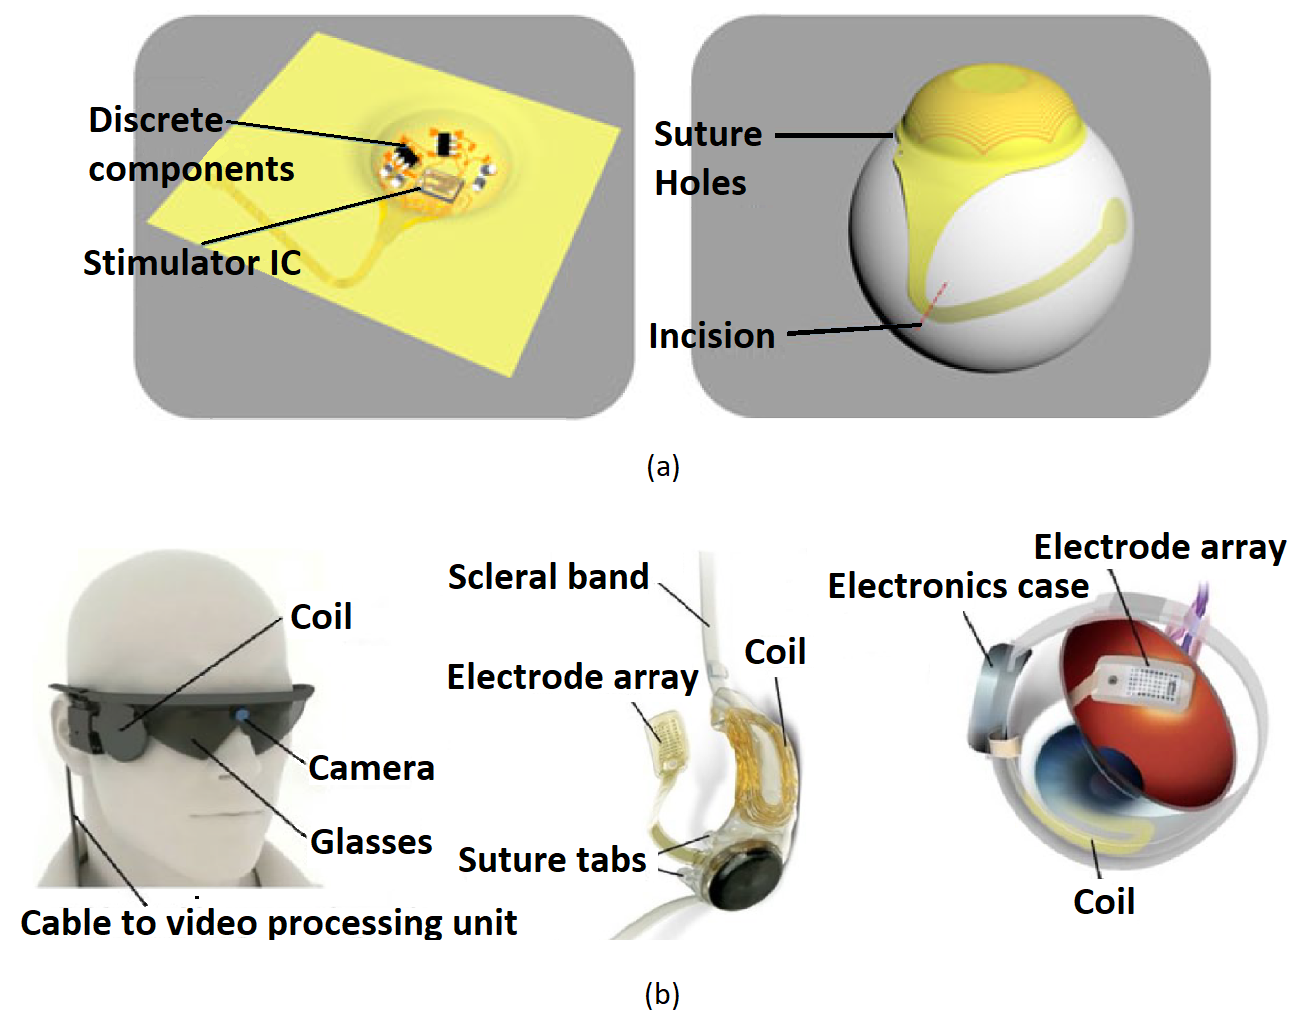
\includegraphics[width=110mm]{Figure/SensoryAid/VICollage}
    \caption{Schematic illustrations and photographs of visual impairment aids. (a) Illustration of LCP packaged monolithic retinal prosthesis system. (b) Illustration of Argus II epiretinal implant system.}
    \label{fig:VICollage}
\end{figure}

The level of visual impairment among individuals varies from moderate to profound and is classified by the Snellen visual acuity scale. In such a scale, the individual with impairment is asked to read individual letters placed a certain distance apart and are given a score compared to the healthy average. For example, 20/60 vision means that the visually impaired individual needs to be 20 feet away to see something that a healthy individual could see from 60 feet. More severe than visual impairment, legal blindness is defined as ``a visual acuity of 20/200 or a visual field of 20 degrees or less" according to the American Foundation for the Blind \parencite{AFB}. 

Visual aids are meant to help individuals suffering from any of the categories of blindness and low vision described above. These aids can be broadly divided into the categories of non-invasive and invasive devices. The former category of devices try to substitute vision with another sensing modality such as hearing. Therefore, range finding sensors such as ultrasonic sensors in conjunction with some form of sensory feedback are frequently used. In contrast, the invasive devices try to improve vision directly. For example, photodiode arrays are used in subretinal implants. 
 
There have been many ATs proposed in the literature recently in the sensory substitution category. One such paper, \textcite{kim_3-d_2020}, describes the use of ultrasonic sensors that are mounted on a glasses-like device to communicate object detection information in the user's field of view via sound. A total of three ultrasonic sensors are used, tilted at a 23$^{\circ}$ angle in the vertical direction with respect to each other to avoid interference. Object proximity to the user is communicated by both pitch and volume. The pitch describes if the object is in the top, center, or bottom of the sensors' field-of-view. The volume distinguishes how far the object is, with 10-step volume resolution. As an example, if the user is going towards the curb of a sidewalk, the sound produced by the device might be a 2-step, $C_3$ pitch sound. In contrast, if the user approaches a perpendicular tree branch at head height at the edge of the sensor's distance detection range, the device would emit a 10-step, $C_5$ pitch sound. 

In the invasive device market, retinal implants have shown efficacy as a long-term solution. \textcite{bloch_advances_2019} identifies three categories of retinal prosthetic devices: epiretinal, subretinal, and suprachoroidal and gives examples of commercial options for each. Epiretinal implants have found the most commercial success. The Argus II device \parencite{SecondSightMedical} consists of an external glasses-mounted camera and processing unit that records the environment as shown in Figure \ref{fig:VICollage}. The recorded image is then sent by modulating the RF power carrier to a coil and implant electronics implanted near the temple. From here the associated stimulus pulses are delivered via a flexible cable to the epiretinal stimulator electrode array that is surgically fixed to the surface of the retina. An advantage of this device is the well-developed surgical procedure. However, the drawbacks lie in the fact that stimulation of neurons behind the retina would require higher stimulation current levels and the device is susceptible to adverse events such as the degradation of the RF link due to misalignment of the coils, which can render the device instantly nonfunctional. Subretinal prostheses are unique because they use a photodiode array to generate photocurrent powered by light hitting the retina. This is in contrast to an epiretinal implant that uses an external camera. Though the photocurrent alone is not enough to elicit retinal stimulation, a simple external power unit can provide the necessary power for this device to be functional. Moreover, since electrodes are closer to the neurons behind the retina, lower levels of stimulation current are required.  

The Alphs IMS and AMS, designed by the company Retina Implant AG that has since gone out of business, are two devices that use the described subretinal implant mechanism. Finally, suprachoroidal prostheses have also been explored by some research groups. Leveraging the vast experience gained from cochlear implants, the Bionic Vision Australia group designed a 24-channel system that was implanted and tested \parencite{BionicVision}. The device showed some promise in terms of improvement in visual acuity; however, there were complications with the surgical procedure. Additionally, due to array distance from the retinal neurons the amount of stimulation current required was relatively high which poses some technical and safety challenges. 

Despite being available commercially since the 1980s \parencite{bloch_advances_2019}, there is still an ongoing research effort in the field of retinal implants targeting deficiencies in currently available devices. One of those deficiencies is the packaging used in epiretinal devices for the stimulator connected to the retina. Following the lead of packaging used in the established field, such as cochlear implants, retinal implants have traditionally used titanium-based encapsulation. The main benefits of this approach are that titanium is biocompatible, corrosion resistant, and has a high strength-to-density ratio. These properties make it a desirable packaging material for implants \parencite{jeong_miniaturized_2015}. Additionally, for cochlear implants that are generally fixed to a point inside a bone behind the ear, the device movement is not a major concern, while it is one of the major drawbacks of using such encapsulation for retinal implants. 

\textcite{jeong_miniaturized_2015} proposes a new polymer-based material for packaging with greater stiffness than a traditional MEMS device but less stiffness than the commercially-used titanium encapsulation. The argument made is that using biocompatible liquid crystal polymer will improve the user experience and the robustness of the solutions because it is conformable to the retinal surface as well as being sturdy enough to withstand the wear and tear associated with being implanted in the body. 

\subsection{Auditory Impairments}
\begin{figure}[h!]
    \centering
    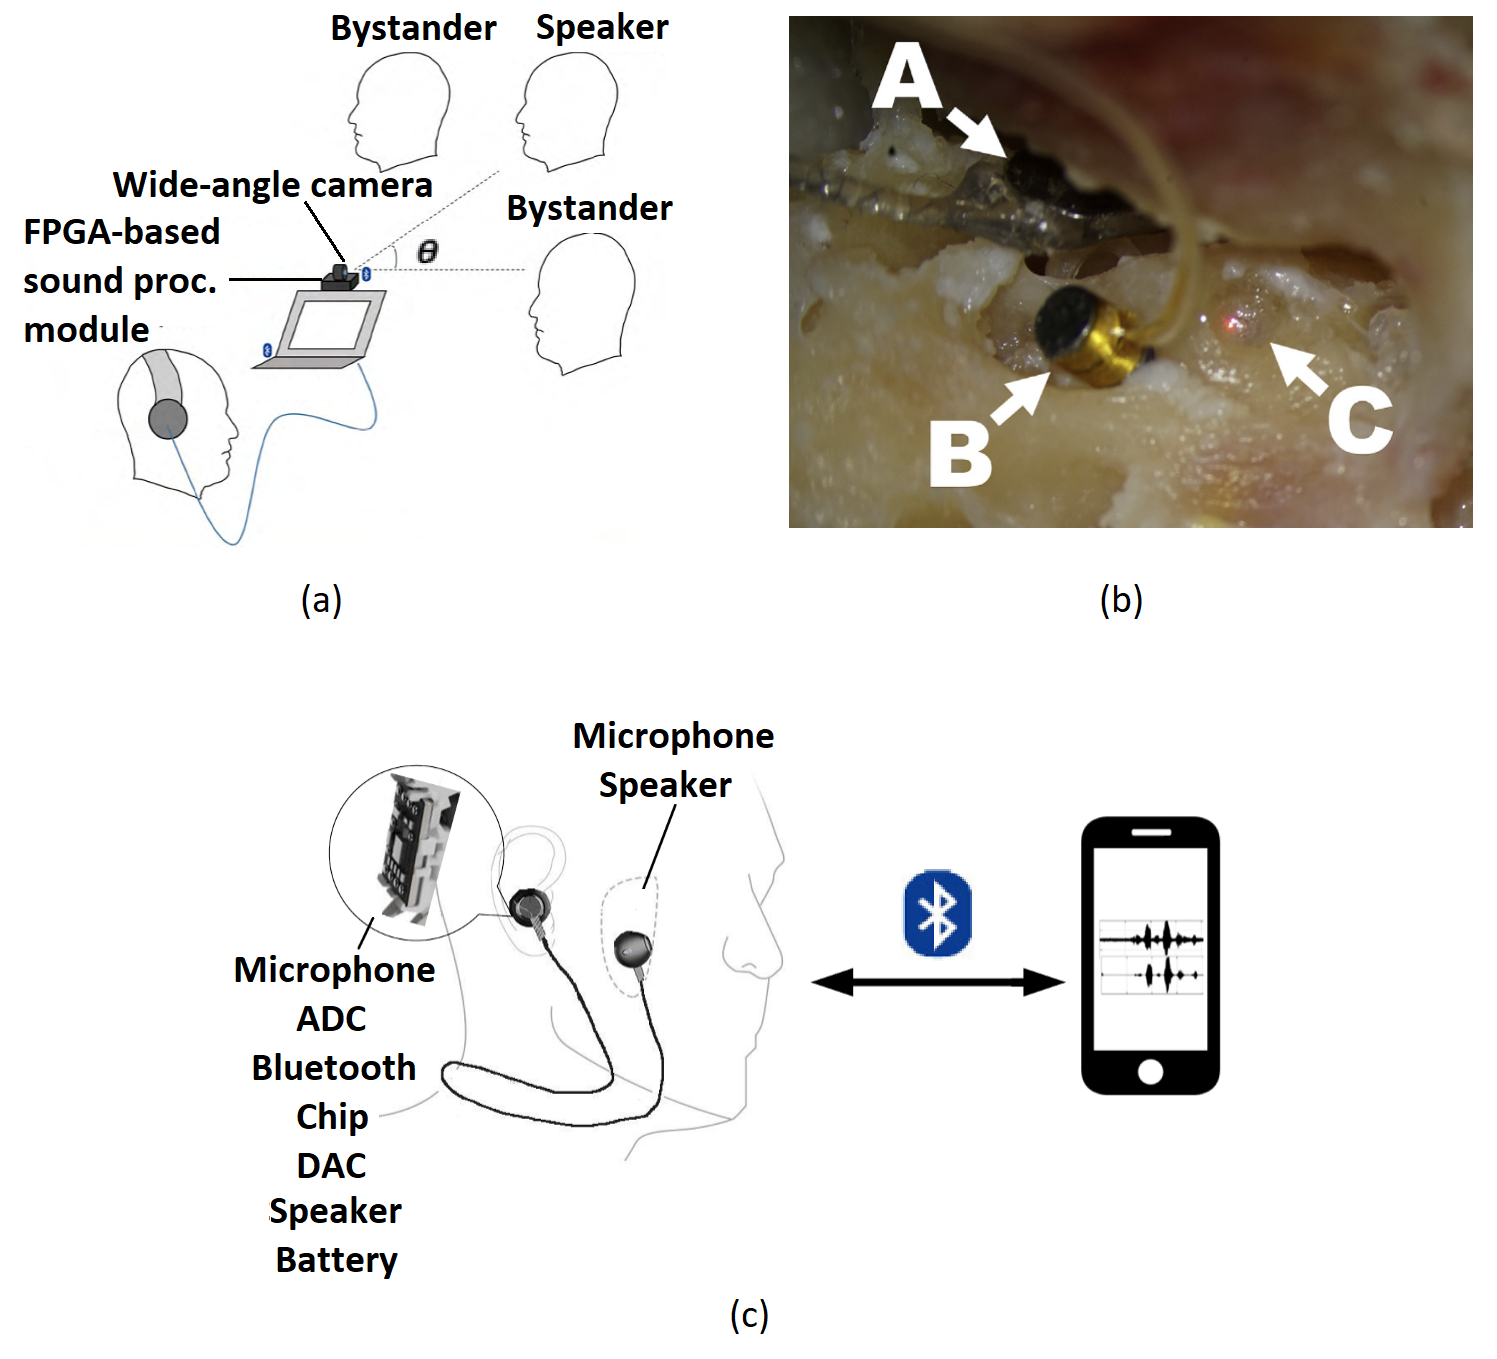
\includegraphics[width=100mm]{Figure/SensoryAid/AICollage}
    \caption{Schematic illustrations and photographs of auditory impairment aids. (a) Illustration of wide angle camera setup to locate and eliminate sources of noise based on spatial differentiation. (b) Photograph of piezoelectric sensor placed in incudostapedial joint as a way to eliminate the need for an external microphone. (c) Illustration of hearing aid system using deep learning algorithms processed on a generic smartphone.}
    \label{fig:SensAidCollage}
\end{figure}
\tab Auditory impairments, like visual impairments, can be classified by their severity. The classification is based on the tone loss. On the low end of the scale, the average tone loss for individuals with first degree moderate hearing loss is 41 dB to 55 dB. On the other extreme, individuals with cophosis (i.e. total hearing loss) have an average tone loss exceeding 120 dB \parencite{IBFA_audiometric_1996}. 

\tab The recent literature regarding auditory impairments suggests the potential solutions under two categories: invasive or non-invasive. In the latter category, external hearing aids are common. Research in this area mainly focuses on improving older designs by taking advantage of modern sensors and signal processing techniques. \textcite{lin_design_2019} tackles the issue of low signal strength in hearing aids by using cameras to locate the speaker and implement an adaptive beamforming method. Adaptive beamforming is a signal processing technique that improves the signal strength in a particular direction by combining sounds from an array of microphones with specific delays. As a result, the beamforming technique can separate noise and signal using spatial information, which is beneficial for improving hearing aid speech intelligibility. The authors propose the use of image processing and machine learning (ML) algorithms to detect where the speaker is and use this information to calculate the difference in time of arrival from different speakers. A field-programmable gate array (FPGA) is used to code the logic that will convert live video from a wide-angle camera into spatial information used in the adaptive beamforming technique. After testing, the proposed system improved the signal-to-noise ratio of sound from a noisy environment by ~5 dB. 

\textcite{li_smart_2020} also takes advantage of ML algorithms; the technique presented uses a smartphone rather than an FPGA to do the processing. The motivation behind this is to take advantage of the ubiquitous nature of smartphones. This proposed device implements a real-time deep learning (DL) algorithm to enhance recorded speech that is then played by the person's hearing aid. The microphone first picks up the sound, which is then transmitted via Bluetooth to the user's smartphone. The smartphone stores the signal in a buffer, which output is processed by the DL algorithm in real-time. With an average delay of 4-6 ms, the data is then transmitted back to the a speaker that plays the sound back to the user. Testing of the device showed that the DL algorithm improved the signal-to-noise ratio by a minimum of 20\%.

Pivoting now to invasive devices, receiving cochlear implants (CI) is a well-established and accepted treatment for hearing loss. As of 2011, over 220,000 individuals worldwide had received CIs according to \textcite{cosetti_cochlear_2011}. This paper reviews commercially available devices and compares them based on several technical features. The three most common commercial CIs including the HiRes devices \parencite{advanced_bionics}, Nucleus devices \parencite{cochlear_nucleus_systems}, and MAESTRO devices \parencite{med_el_2_maestro}. Mainly, the focus is on the most recent efforts of these companies to improve their respective devices to get better spatial specificity within the cochlea. A number of factors limit this specificity, including inner ear fluid that moves the stimulator, interference between adjacent electrode sites, and the distance between the stimulating electrode and the ganglia neurons. 

The HiRes CI series uses a Fidelity 120 \parencite{advanced_bionics_fidelity120} processing strategy that uses current steering to not only reduce adjacent electrode interference, but to also create "virtual" channels. Additionally, a preprocessing strategy implemented prior to the transmission to the implanted stimulator works to reduce noise immediately following recording by the microphone. As a result, the HiRes devices have shown better pitch and tone discrimination, directly related to improved speech perception. The Nucleus devices also use processing and preprocessing steps. The preprocessing step improves the audio source by using an adaptive directional microphone. Going further, a special modiolar-hugging electrode is used that helps physically space out the electrodes in the most optimized manner while maintaining closeness to the ganglia neurons. The processing step eliminates duplicate or masked sounds before stimulation. Finally, the MED-EL MAESTRO line of devices uses simultaneous stimulation of cochlea sections to improve speech perception versus the traditional sequential approach. Like the previous device, a custom FlexEAS electrode is used to appropriately space the electrodes while having the added benefit of maintaining existing inner ear functionality. Similar to the Nucleus devices, the MED-EL devices also use titanium packaging for stimulators rather than ceramic ones to reduce the size and increase usage in pediatric users.

Current research in the field of CIs explores ways to improve an established technology. \textcite{esinger_sensor-actuator_2019} looks at how to make a CI fully implanted by omitting the external microphone in exchange for a Floating Mass Transducer (FMT). The operating principle of the FMT is to record external sound by picking up vibrations in the long process of the incus. The vibrations are converted into a sound signal through the use of a piezoelectric sensor that is surgically placed in the incudostapedial joint. With this modification, the CI would be completely implanted in a single surgery, which could be beneficial for users who find it inconvenient to have a bulky external microphone placed on the side of their head. In this prospective device, an inductive link could be used to power the device. 

\subsection{Sensors in Use}
\tab In this section, we will explore some of the sensors unique to this area of sensory a devices in more detail.

\subsubsection{Photodiode Array}
A photodiode is essentially a PN junction where the P+ and N+ substrates are separated by a depletion region formed through the combination of holes and electrons. The size of the depletion region is affected by the magnitude of a reverse bias voltage applied to the diode. When light strikes the diode with a wavelength of less than 1100 nm \parencite{ida_sensors_2013} to exceed the bandgap energy of silicon, the electrons in the valence band are energized and move to the conduction band causing the current to flow. The amount of light striking the photodiode is therefore directly proportional to the amount of current generated. In \textcite{bloch_advances_2019}, subretinal implant devices are described that use photodiode arrays placed directly on the retina to generate photocurrent from light entering through the pupil.

\subsubsection{Piezoelectric Sensor}
The piezoelectric effect is a phenomenon where specific types of material (e.g. quartz, topaz etc.) produce an electric charge proportional to the mechanical stress applied to them \parencite{ida_sensors_2013}. Furthermore, the geometric strain of these materials is proportional to changes in the applied electric field. In \textcite{esinger_sensor-actuator_2019}, the authors use a sensor made of a piezoelectric material to remove the external component of the CI by converting the vibrations caused by sound in the long process of the incus into charge. By doing this, the piezoelectric sensor replaces the functionality of a microphone.


\section{Seating and Mobility Aids}

Seating and mobility aids cover a broad spectrum of assistive technologies such as wheelchairs, scooters, walkers, canes, and crutches. These technologies aim to enhance the mobility and in turn quality of life of the user by helping the control of head, arms and hands, ensuring an improved body stability for ease of movement. Further advanced seating and mobility applications make use of sensors attachable to the assistive technologies that improve the effectiveness of these tools. Some of the most popular applications are smart chair, smart walker/cane, and smart bed. While the target population for these applications is mostly the people with physical impairments and seniors, applications such as the smart bed would also help analyze able-bodied individuals' behavior to avoid possible future health problems \citep{laurino_smart_2020,su_monitoring_2019}. The common characteristic of these applications is that they are equipped with sensors that collect the physiological data both from the user and the environment to monitor and control the user's surroundings. \\

\subsection{Smart Chair}

People with severe physical disabilities are highly dependent on their powered mobility means to go from point A to point B either within their home environment or outside. Not unlike the automotive industry, in the past decade, wheelchair technologies have been advanced, and now evolving from the power wheelchairs (PWs) to smart wheelchairs (SWs) \parencite{leaman_comprehensive_2017}. Traditional PWs require the users to navigate the wheelchair using a hand-rim or a joystick, which may not be accessible by severely disabled users. SWs equipped with advanced assistive technologies, such as human-computer interfaces, sensor arrays, sensor processing algorithms, and machine-vision, have been developed to provide mobility and improved living conditions to those users. SWs not only advance the control and navigation mechanisms of the wheelchair but also elevate the user comfort level as well as usability and safety of the wheelchair in various environments (e.g. indoors, outdoors, rugged train, sloped curbside, etc.) \parencite{ahmad_screen-printed_2019,hu_smart_2020,tavares_wheelchair_2020}.

%In the literature, 
The general approach for developing SWs is to deploy sensors and data processing units to PWs for collecting and analyzing a much wider range of inputs from the user and the environment \parencite{leaman_comprehensive_2017}. The commonly preferred method for controlling and navigating the wheelchair is haptic feedback, which uses various tactile sensors equipped with force sensors \parencite{hadj-abdelkader_haptic_2012,morere_haptic_2015,poorten_powered_2012,trujillo-leon_tactile_2018}. A haptic handlebar using force-sensing resistor sensors (FSR) is proposed in \textcite{trujillo-leon_tactile_2018}. The tactile sensor-based steering, demonstrated in Figure \ref{fig:smart_chair}.a, aims to assist caregivers in navigating the wheelchair. The handlebar is equipped with a matrix of FSRs; the force applied to the handlebar changes the resistivity of the FSRs. The variation in the resistance is converted to voltage by transimpedance amplifiers. The voltage outputs are then digitized by an analog-to-digital converter (ADC) and sent to a personal computer (PC) via a universal serial bus (USB) connection. The digitized output values coming from the sensor matrix compose a pressure map used to control the motion of the wheelchair. 

Being seated for long hours in a wrong position can cause secondary disuse problems such as pressure sores \parencite{redford_seating_1993}; therefore, monitoring the user's sitting posture is critical. \textcite{sen_wireless_2018} proposes a wearable sensor patch that monitors the contact pressure continuously for pressure ulcer prevention. The sensor patch utilizes FSRs for measuring the contact pressure. In \textcite{tavares_wheelchair_2020}, fiber Bragg grating (FBG) sensors are used to detect higher pressure areas during seating to prevent the development of pressure ulcers in wheelchair users. The system is based on the principle that the reflected Bragg wavelength in an optical fiber changes with the variations in fiber strain caused by the pressure as shown in Figure \ref{fig:smart_chair}.b. In the implementation, six FBGs are embedded into a thermosetting epoxy resin cylinder to maintain the fiber's physical integrity and placed in different points on the wheelchair where pressure is applied the most, such as scapulas, ischiatic zones, and heels. Two other FBGs are inserted in separate optical fibers for temperature monitoring; the purpose of temperature monitoring is to analyze the thermal influence on the pressure values since the reflected Bragg wavelength also shifts with temperature variations. 

\begin{figure}[t!]
    \centering
    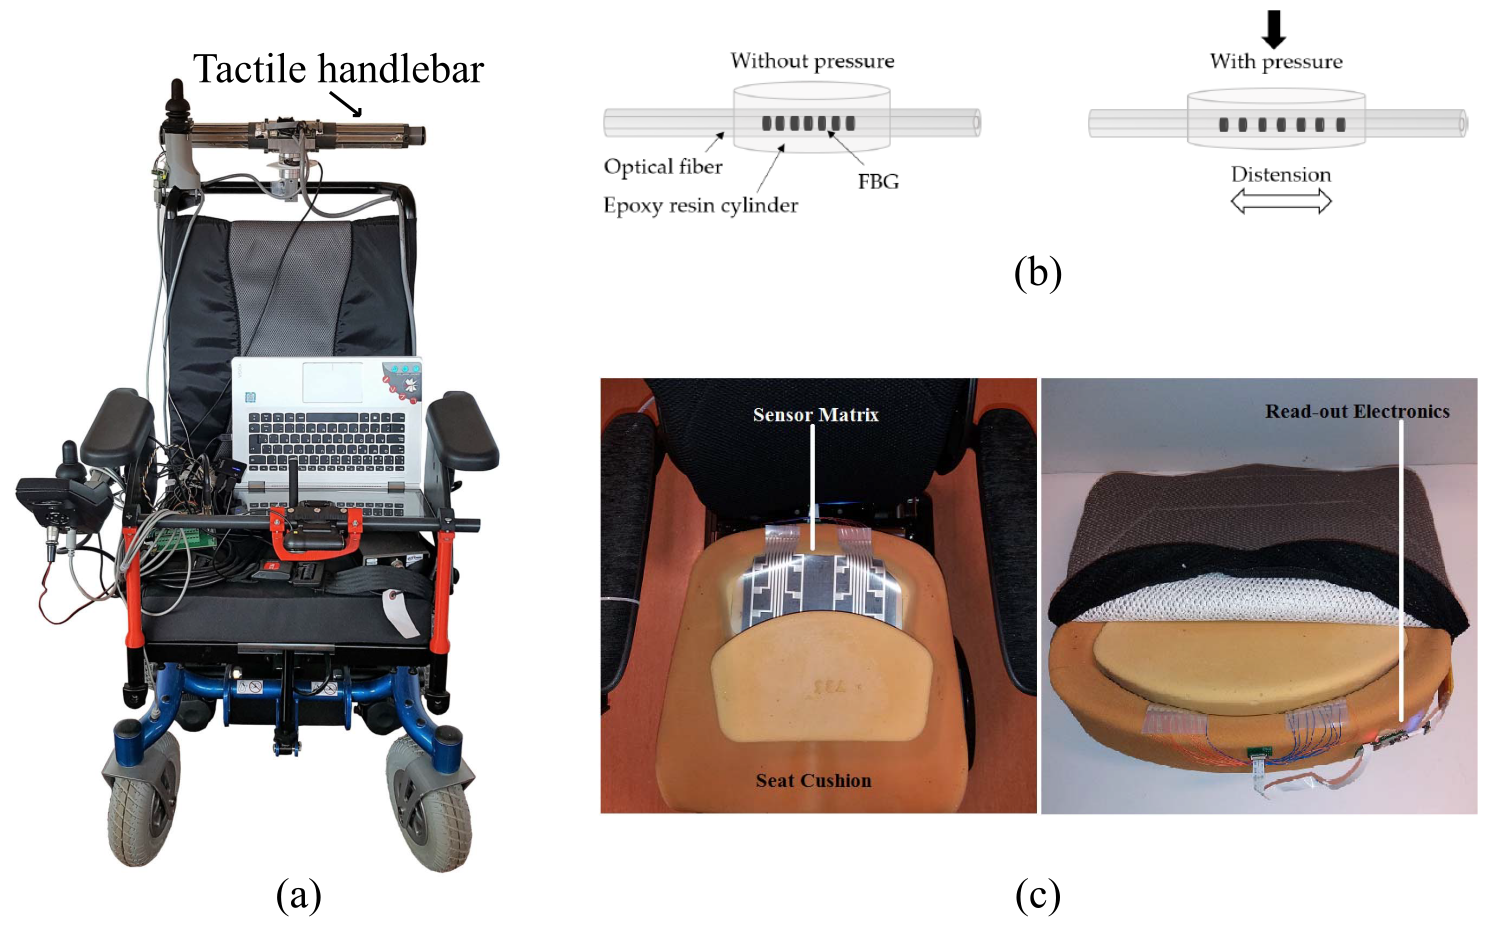
\includegraphics[scale=0.95]{Figure/Seating and Mobility Aids/Smart_chair.PNG}
    \caption{Illustrations from the SW applications. (a)  Setup of the wheelchair with tactile sensor-based steering, modified from \parencite{trujillo-leon_tactile_2018}. (b)  Effect of pressure on the physical structure of the FBG-based pressure sensor, reproduced with permission from \parencite{tavares_wheelchair_2020}.(c) Placement of the pressure sensors in the seat cushion,reproduced with permission from \parencite{ahmad_screen-printed_2019}. }
    \label{fig:smart_chair}
\end{figure}

\textcite{ahmad_screen-printed_2019} presents a screen-printed sensor that measures the pressure distribution on the seat of a wheelchair. The screen-printed sensor consists of 16 piezoresistive sensing elements printed on a polyethylene terephthalate sheet in the form of a $4\times4$ sensor matrix. The sensor matrix is placed underneath the seat cushion, as can be seen in Figure \ref{fig:smart_chair}.c. The data collected from the sensors is sampled using 16 dedicated ADC channels that have a 10-bit resolution. The sampled data is sent to a PC by a Bluetooth module on-board and is processed using MATLAB. \textcite{hu_smart_2020} demonstrates a smart chair design that monitors the user's sitting posture to ensure a healthy seating position by using flex sensors and a field-programmable gate array (FPGA) implemented neural network. The flex sensors, which are sensitive to bending, are placed on an office chair's back and seat. The sensor output is fed into an Arduino microcontroller and a separate ADC module for sampling, outputs of which are given to a PC and an FPGA, respectively. The sampled data received by the PC is used for training the neural network, and the data received by the FPGA is utilized for validation.

\subsection{Smart Walker/Cane} 

%Technology-assisted canes can be equipped with single or multiple sensors depending on the system requirements and operating conditions. 
In the literature, ultrasonic sensors, infrared (IR) sensors, camera, accelerometer, gyroscope, humidity sensor, global positioning system (GPS), which can be considered an outdoors position sensor, are widely employed in the technology-assisted canes \parencite{khan_technology-assisted_2018}. For instance, ultrasonic sensors and cameras are used to detect and recognize objects, while IR sensors are utilized to estimate the distance and stair inclination. The accelerometer detects the steps; the GPS localizes the cane user; the gyroscope detects the cane's orientation \parencite{ahmad_multi-sensor_2018,leal-junior_plane-by-plane_2019,wade_feasibility_2019}.

\textcite{wade_feasibility_2019} presents an instrumented cane system that collects mobility data and assesses the fall risk with the sensors attached to the cane. Force sensing resistors and a 9 degrees of freedom (DOF) inertial measurement unit (IMU) are placed on the cane handle to detect how much grip pressure the user is applying. Afterward, pressure data can be used to figure out potentially harmful usage. The cane's shaft has an RF module that transmits the data from the sensors to a custom dongle and an ultrasound sensor that detects an obstacle. A single-axis load cell is located at the base to measure the weight borne on the cane. A 3DOF accelerometer, also at the base of the cane, is used to measure the linear acceleration. The data collected from the sensors is fed into ADCs, also placed on the cane. Later, the sampled data is sent by the RF module to a PC for processing. 

A standard walker is equipped with load cells and a light detection and ranging (LIDAR) sensor to monitor the walker's usage in \textcite{viegas_monitoring_2018}. The load cells, attached to the walker's base, as shown in Figure \ref{fig:smart_cane}.a,sense the applied force on the walker's legs. The data coming from the cells is analyzed to find the center of mass information. The LIDAR sensor measures the distance traveled by the user and walker. The gathered data is used to monitor the separation between the user and walker, and hence accordingly, the coordination between the walker's movement and the user's gait. The sensor data is collected by a microcontroller and transmitted to a PC, in which an on-board Bluetooth module processes the data. In the data processing part, two risk factors are identified. The first risk factor is based on the balance of forces applied on the walker's legs, and the second one is based on the coordination between the walker's movement and the user's gait. The risk factors are computed using the sensor data. A graphical user interface (GUI) is created to monitor both the sensor data and risk factors in real-time.

\textcite{meshram_astute_2019} proposes a cane that can detect obstacles, familiar objects, and wet floors in the environment to assist visually impaired people. The obstacle detection is achieved by utilizing five ultrasonic sensors on different locations of the cane's shaft. At the top of the cane, the radio-frequency identification (RFID) reader recognizes the objects with an RFID tag in the environment.
% Because of the tag's location, the system cannot identify the unfamiliar (non-tagged) objects, which is a downside of the system that needs to be improved. 
At the base of the cane, a liquid contact sensor detects the wet floors. The placement of the sensors is shown in Figure \ref{fig:smart_cane}.b. The sensor data is processed on a small computer located on the cane's body. After processing the sensor data, the smart cane provides information to the user about the obstacles and objects in the environment through tactile feedback using the vibrator at the cane's handle or auditory feedback using wired/wireless headphones. 

\begin{figure}[h!]
    \centering
    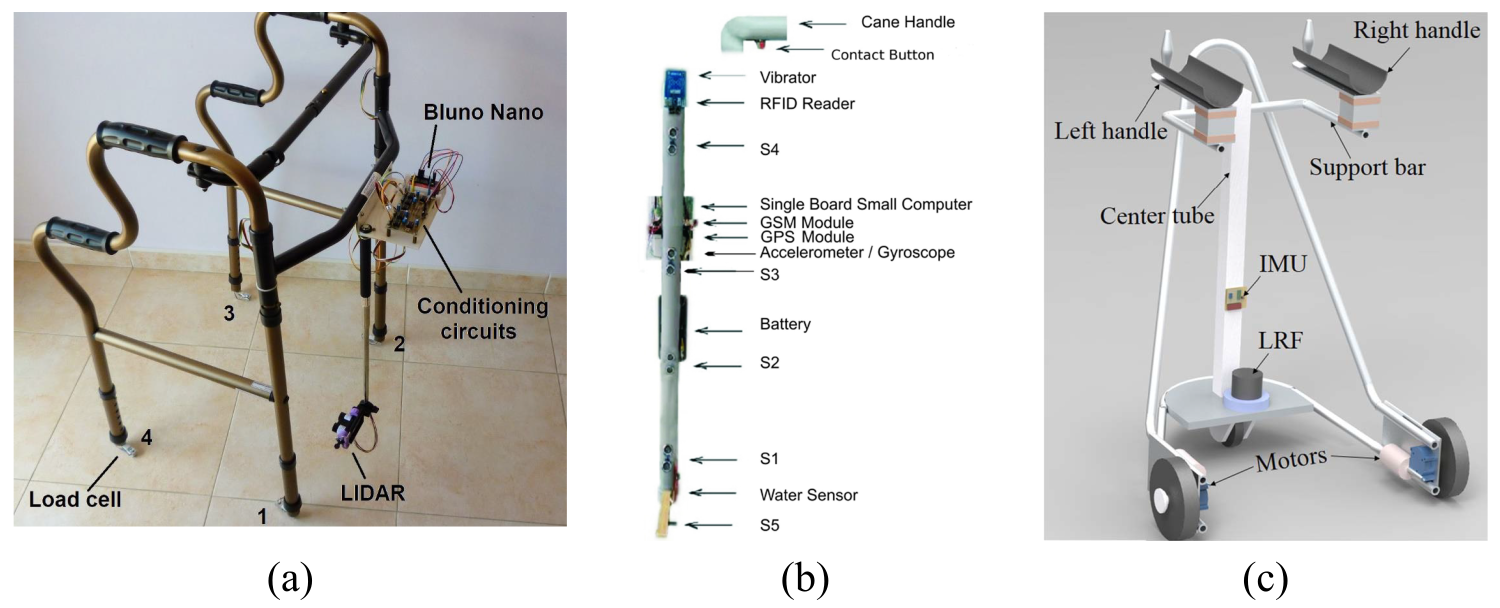
\includegraphics[scale=0.95]{Figure/Seating and Mobility Aids/Smart_cane.PNG}
    \caption{Illustrations of smart walker/cane applications. (a) A standard walker equipped with load cells and a LIDAR to assist the user, from \parencite{viegas_monitoring_2018}, (b)  A cane with various sensors that aims to guide visually impaired people, reproduced with permission from \parencite{meshram_astute_2019}, (c) Overview of the SW used for the fiber Bragg grating (FBG) array implementation, FBG array is placed on the support bar. Reproduced with permission from \parencite{leal-junior_plane-by-plane_2019}.}
    \label{fig:smart_cane}
\end{figure}

A fiber Bragg grating (FBG) based smart walker is presented in \textcite{leal-junior_plane-by-plane_2019}, which can monitor the temperature, strain, and vibrational oscillations to estimate the gait cadence, the floor vibration condition, and the force applied to the walker by the user. The working principle of the FBG sensors is based on the shift of the Bragg wavelength due to temperature variations and strain. Five FBGs are placed on the walker's support bar to capture the force applied by the user and vibrational oscillations due to the floor level variations. In order to evaluate the data obtained by the FBGs, the authors deployed force sensors in the walker's handle, an inertial measurement unit on the walker's shaft, and also a laser range finder at the walker's base, as shown in Figure \ref{fig:smart_cane}.c, to compare force measurements, vibrational oscillations, and gait cadence data, respectively.

\subsection{Smart Bed}

Continuously monitoring the vital sign parameters such as blood pressure, cardiac and respiratory rates is of great importance to detect cardiac and respiratory diseases at an early stage and assess sleep quality. The gold standard for monitoring the vital signs during sleep is the polysomnography method \parencite{jafari_polysomnography_2010}, an obtrusive method, which is not suitable for use in home settings. Hence, the recent research in smart bed applications is focused on unobtrusive methods that can be employed both in a professional setting and a home-care environment \parencite{laurino_smart_2020,su_monitoring_2019,waltisberg_detecting_2017,wang_noninvasive_2020,yu_multi-modal_2019}. 

These applications rely on noninvasive sensor technologies generally placed in the bed mattress. These sensors can create the pressure map of the body, which provides information on respiratory and cardiac rates when continuously generated by utilizing piezoresistive, capacitive, optical, and piezoelectric sensors \parencite{laurino_smart_2020,waltisberg_detecting_2017,wang_noninvasive_2020}; ballistocardiography is another popular method to measure blood pressure and heart rate \parencite{su_monitoring_2019,yu_multi-modal_2019}. There are also applications in which the sensors are located around the smart bed setting to measure respiration; camera sensors, ultrasonic proximity sensors, multi-walled carbon nanotubes sensors are among the frequently used sensor solutions for such applications.

\textcite{laurino_smart_2020} proposed a smart bed with multi-modal sensing for the assessment of sleep quality based on multiple parameters. The data for the assessment is collected from two different sensor interfaces. The first interface collects information from the user's body, and it is called physiological data collector (PDC). The second interface gathers data from the environment, and it is called environmental data collector (EDC). The PDC is equipped with textile pressure arrays (piezoresistive sensors), lied on the bed, as demonstrated in Figure \ref{fig:smart_bed},  and tri-axial accelerometers, also placed on the bed, for monitoring the position, movement, breath, and heart rates of the user. The ability to detect position, movement, breathing and heart rate simultaneously is the key specification of the proposed smart bed, which differentiates it from the other literature that provide single mode solutions. The EDC has sensors that collect sound intensity, temperature, relative humidity, and luminosity data from the environment. The sensor data coming from the EDC and PDC sensors is processed in a docking station. A sleep-quality algorithm generates a global sleep-quality index that  assesses the sleep quality of the user. 

\begin{figure}
    \centering
    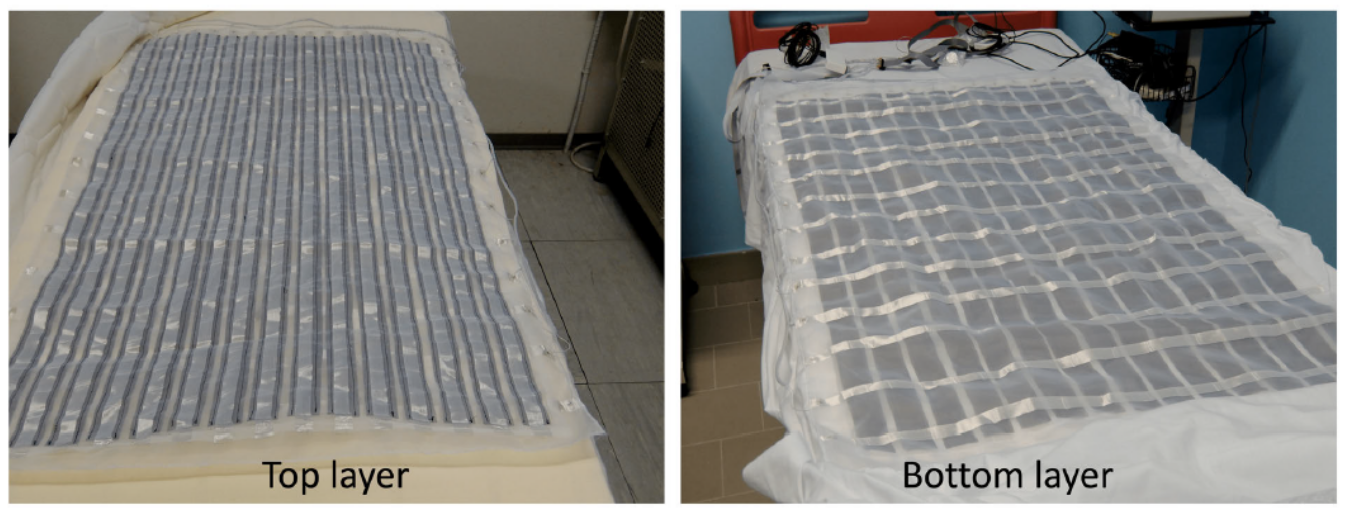
\includegraphics[scale=1]{Figure/Seating and Mobility Aids/Smart_bed.PNG}
    \caption{Textile pressure mapping system based on a textile resistive matrix with 13 column conductors and 15 row conductors for a total of 195 sensing areas, from \parencite{laurino_smart_2020}.}
    \label{fig:smart_bed}
\end{figure}

In another study, an array of strain gauges placed between the bed mattress and the bed frame to sense the pressure variations on the bed mattress to monitor the user's body movements and respiration \parencite{waltisberg_detecting_2017}. The aim of monitoring these body signs is to understand the sleep-related breathing and movement disorders and guide the treatment procedure. The sensor array is composed of eight uniformly distributed strain gauges, and the total size of the array is 72 cm by 16 cm, which covers the whole width of the bed. Two fusion methods were applied in the processing of the sensor data, namely measurement and decision fusion; both methods include filtering, feature extraction, normalization, and classification algorithms. 

\textcite{wang_noninvasive_2020} presents a smart mattress that can be used for household and hospital health monitoring. Optical fiber Mach-Zender interferometer (MZI) senses the pressure variations due to cardiac and breathing activities; sensor outputs are then processed and analyzed to generate information about the user's health status. The optical fiber MZI is composed of a laser source, couplers, single-mode fibers, and photodetectors. In the proposed design, the sensing arm is placed in the mattress, and reference fiber is arranged in a separate terminal box. The optical phase difference between the reference and the sensing fibers is proportional to the signal path length of these fibers. When a pressure is applied on the mattress, the path length of the signal travelling in the sensing fiber changes that varies the phase difference between the reference and sensing fibers. The photodetectors can read the variations of the phase difference at the outputs of the optical fiber MZI. The raw pressure variation data is used to extract the cardiac activity information after passing through several processing steps. 

\textcite{su_monitoring_2019} demonstrates a smart bed system that utilizes hydraulic pressure sensors placed underneath the bed mattress to identify two ballistocardiographic (BCG) measures, namely ballistocardiogram pulse strength (BPS) and ballistocardiogram pulse deviation (BPD). The purpose of identifying these metrics is to monitor the blood pressure, which can be used to signify the risk of cardiovascular disorders at an early stage and prevent them. 

\textcite{yu_multi-modal_2019} presents a multi-modal sensor that is a combination of a capacitive electrocardiogram (cECG) electrode, reflective PPG (rPPG), and magnetic induction (MI) sensor for unobtrusively monitoring the vital parameters of the human body, namely the heart and respiration rates. The cECG uses the same principles of a standard ECG to monitor cardiac activity. However, unlike the standard ECG, cECG does not require direct contact with the human skin and can detect the cardiac signals through the layers of various materials such as clothing. The multi-modal sensor integrates the rPPG and MI sensors into the cECG electrode to enable data fusion. The rPPG and MI sensors measure the heart and the respiration rates and complement the measurement data obtained from the cECG electrode to increase the measurement's reliability.


\subsection{Sensors in Use}

\subsubsection{Pressure Sensors} 

Pressure sensors are the most popular type of sensors used in seating and mobility aids. One can classify the pressure sensors according to the sensing principle employed. In this section, 3 classes of the pressure sensors are discussed namely piezoresistive, fiber-optical, and hydraulic sensors. %Pressure sensors can be classified into 3 groups namely the piezoresistive, fiber-optical, and hydraulic sensors.



Flexible semiconductor materials, which resistivity changes with shape deformation (bending, stretching, and compression), are classified as piezoresistive materials \parencite{morris_chapter_2016}. Piezoresistive materials are widely used for force sensing in seating and mobility aids. \textcite{trujillo-leon_tactile_2018} utilizes rectangular force-sensing resistors (FSRs), which are basically piezoresistive sensors. In this application, FSRs are placed on the handlebar (diameter 42.5 mm, length 120 mm) of the wheelchair to detect the force applied by the user on the handlebar.

Piezoresistive sensors (17 mm x 12 mm x 350$\mu$m) screen-printed on a polyethylene terephthalate substrate measure the pressure distribution on the wheelchair seat \parencite{ahmad_screen-printed_2019}; the sensor is capable of sensing 0.1 - 100 N of force. Force sensing resistors with a sensitivity range of 0.2 - 20 N are attached to the cane handle for measuring the grip pressure in \textcite{wade_feasibility_2019}.\textcite{laurino_smart_2020}  mapped pressure by 195 evenly spaced (separated by 3 cm in the rows and 8 cm in the columns) textile piezoresistive sensors made of CARBOTEX 03-82 fabric. \textcite{hu_smart_2020} uses a piezoresistive sensor, called flex sensor, composed of a  polymer ink with conductive particles and plastic flake for pressure sensing. The sensor is 73.7 mm long, has 64.5 mm width and 0.5 mm thickness.

The reflected Bragg wavelength of the FBGs is a pressure and temperature-dependent parameter \parencite{tavares_wheelchair_2020}. Thus one can detect pressure variations by monitoring the change in the reflected Bragg wavelength with compensating for the temperature changes. The fiber optical sensor in \textcite{tavares_wheelchair_2020} comprises six FBGs placed in an epoxy resin cylinder of 2 cm diameter for monitoring the pressure in six different locations on the wheelchair. \textcite{leal-junior_plane-by-plane_2019} utilizes FBGs with 1.57 \pm 0.15  pm($\mu\epsilon^{-1}$) strain sensitivity for sensing the applied force on the walker handle. Unlike the FBG approach, the system in \textcite{wang_noninvasive_2020} is based on MZI with two fiber arms, namely the reference arm and sensing arm. The pressure applied to the sensing fiber increases the path in which the light travels and creates a phase difference between the reference sensor and the sensing sensor, proportional to the amount of pressure.

Hydraulic sensors transduce pressure to an electrical signal and can be used to monitor the relative blood pressure in a smart bed setting \parencite{su_monitoring_2019}. The commonly used hydraulic sensor type is the strain gauge \parencite{waltisberg_detecting_2017}, which produces a variable electrical signal proportional to sensor's elastic deformation.


\subsubsection{Inertia Sensors}

Accelerometers, load cells, and IMUs are frequently-used inertia sensors. Inertia sensors in seating and mobility applications are utilized for position and movement detection \parencite{laurino_smart_2020,viegas_monitoring_2018,wade_feasibility_2019}.

\subsubsection{Range Sensors}

Range sensors are used for obstacle detection, navigation and path detection in smart chair and walker/cane applications. Ultrasound sensors  \parencite{meshram_astute_2019,wade_feasibility_2019} and LIDAR sensors \parencite{viegas_monitoring_2018} are the two widely used range sensors. 

%%%%%%%%%%%%%%%%%%%%%%%%%%%%%%%%%%%%%%%%%%%%%%%%%%%%%%%%%%%%%%%%%%%%%%%%%%%%%%%%%%%%%%%%%%%

\section{Manipulation and Control of the Environment}

To provide a convenient tool for people with severe injuries, who cannot carry out everyday tasks using their hands, manipulation and control of the environment has became a popular research topic in the field of assistive technologies. Aside from traditional means, such as joysticks and modified switches, that need a certain level of physical movement ability in the users' hands and fingers, to address this need, two important applications stand out among the others; tongue drive systems and eye-trackers.
%for disabled people without functioning fingers and hands. 

These applications have a wide range of users with high level physical disabilities, such as those with high-level spinal injury, upper limb amputation, amyotrophic lateral sclerosis (ALS), and certain types of stroke. The common characteristics of these applications are that they all use sensors to infer the user intentions from their remaining volitional movement abilities, not in their hands and fingers but and exploit the movements of the tongue and eyes to stimulate the behaviors of fingers and hands.

\subsection{Tongue Drive System}
Mouth and particularly the tongue are inherently capable of sophisticated motor control and high-resolution manipulation tasks with many degrees of freedom thanks to the myriad of sensory and motor neurons that represent them in the human brain. A tongue-computer interface called Tongue Drive System (TDS) was introduced by (Jia Wang et al., 2008) in 2008. The proposed TDS takes advantage of tongues' dexterity and its direct  connections with the brain through the hypoglossal nerve. TDS is envisioned to help people with severe disabilities to conduct their daily activities, including computer/smartphone access, control of the wheelchair and motorized bed. Although promising, the success of a TDS relies on the accuracy of tongue motion tracking. Therefore, the precise localization of the tongue appears to be one of the main research topics for TDS. Magnetic, inductive, and optical sensors have found usage in recent research on localization and tracking of the tongue movements. In the following we elaborate on the use of sensors in some variations of the TDS.

(Sahadat et al., 2018) proposed a multi-modal tongue drive system (mTDS) that deployed magnetic sensors to emulate mouse cursor clicks  by monitoring the tongue movements. Magnetic sensors measuring magnetic field density are used to estimate the location of a permanent magnetic tracer through the mathematical formula mentioned in (Sebkhi et al., 2018). Thus, the raw data from magnetic sensors is processed in real time to track the tongue movements wirelessly with millimeter resolution while maintaining safe use inside the oral cavity without impeding the tongue's natural motion. The system integrates an array of two modules, each of them housing two magnetic sensors, for the measurement of magnetic field density with high accuracy. The tongue's left movement represent a "left click" and right movement represent a "right click". Furthermore, the researchers run an experiment with fifteen healthy subjects. Subjects performed an email typing task with random content via the mTDS versus a keyboard and a mouse. The task included mouse clicking command, and all the subjects could click correctly by using their tongues via the mTDS.

%insert the TDS pictures Magnetic_TDS, Inductive_TDS, Optical_TDS.


Another study (Struijk et al., 2017) utilizes inductive sensors in a tongue-computer interface (TCI) designed for individuals with tetraplegia, which indicates paralysis in all four limbs and torso. The inductive sensors used in the interface design are composed of an array of air-cored inductors. Based on Faraday's law, when a small ferromagnetic tracer that is attached to the tongue is placed at the center of an inductor, the  relative magnetic permeability of the coil increases. Accordingly, the voltage drop across the inductor will increase and maintain that value until the tracer is removed. Relying on this principle, the system scans the inductors and detects the tongue position based on the inductor, which value is changed, and transmits the sensor data through radio to a PC or any other target device. The TCI designed with 18 inductive sensors is placed in the oral cavity. Ten of these sensors construct a 10-key pad, and the rest form the mouse/joystick pad. The TCI embedded the sensor array PCB, a control unit and a battery under user's tongue. The study also presents experimental results that are conducted with two tetraplegic and two able-bodied individuals, who wore the proposed TCI. The maximum typing rates are recorded as 1.8 and 1.4 seconds for repetitive typing of a correct character on the keypad and the mouse pad area, respectively. 


Previous examples were assistive technologies that require a tracer attached to the user's tongue. An example of a tracer-free approach tracks tongue movement based on glossokinetic potentials (GKP), which are potential alterations in electroencephalography (EEG) signals when the tongue touches the side of the cheeks (Nam et al., 2016). GKP used to be described as a signal artifact that should be removed during the preprocessing stage of the EEG signals. In 2012, (Attarian et al., 2012) discovered the relationship between tongue movements and GKP levels. The authors describe the change in GKP levels with the direction of the tongue movement;  when the tongue moves to one side, GKP levels on that side decrease, and vice versa on the other side. The tongue-machine interface (TMI) proposed in this study translates GKP levels into the horizontal position of the tongue with a linear model. EEG electrodes are used to monitor GKP levels changes. The experiment is performed with four subjects. Based on four subjects' 90 random angle cues from $- 90^{\circ}$ to $+ 90^{\circ}$, the TMI's detection mean value of angle is $18.9^{\circ}$. This value is sufficient to control a wheelchair to change the direction angle. The usability of GKP levels is demonstrated and an application to control the direction of powered wheelchair is presented too. %Further research on this topic is going to improve the sensitivity and implement this system on other complicated manipulation tasks. 

Another tracer-free TDS is implemented with four optical distance sensors and one ambient light sensor in (Jiang et al., 2020). While four optical distance sensors over the user's upper jaw detect any contacts with the tongue, the ambient light sensor on the retainer's frontal surface  indicates whether the mouth is closed. This system also includes a sensor data fusion algorithm to eliminate unintended tongue contacts with sensors. The experiments involve eleven healthy individuals to test the discrimination of unintended tongue contacts with new sensor setup and masking ability of the data fusion algorithm. The accuracy of mouth cursor commands on a computer was also tested. The experiment results revealed that the fusion algorithm could mask 86.99\% unintended tongue contacts during swallowing, while the proposed system achieved 97.16±0.94\% accuracy during the random mouth cursor commands test. %This paper presents a functioning tracer-free TDS by using optical sensor with sensor data fusion algorithm to avoid unintended touch.



\subsection{Eye-trackers}
Eye-tracking is the mechanism behind another group of assistive technologies that offer accurate control commands to people with severe disability without requiring any physical interaction. Similar to tongue movements, voluntary eye blinking and movements can be used as a control method for those with a wide range of injuries and diseases ranging from high-level paralysis to progressive diseases like Amyotrophic Laternal Sclerosis (ALS). In the past two decades, many studies have been conducted on eye-trackers and eye-computer interfaces (ECI) that control expansive applications, such as wheelchair, smart home, and office tools. There are even commercial eye-tracking systems available in the market for assistive technology as well as research on the eye motion and evaluating user response to the arrangement of scenes, web pages, advertisement, etc. Tobii series, SR Research and SMI RED250. The following paragraphs will cover several popular eye-trackers based on electrooculography (EOG), infrared camera, microwave resonator and inductive sensors. 

%insert the ET pictures EEG_Wearing, Inductive_Eye 

% EOG Sensory 
Sensory EOG is a method that measures the corneo-retinal standing potential to map the eye's position. A pair of EOG electrodes are placed on the face closed to eyes. When the eye moves towards one electrode, and far from the other one, the corneo-retinal standing potential develops.  Once recorded, post-processing technics can translate these signals into eye movements. A successful implementation of EOG is demonstrated in (Zhang, 2018). In that study, researchers developed an EOG-based human-computer interface (HCI) that controls smart home equipment to help people with severe spinal cord injury. The user sent the control command by blinking an eye towards the corresponding flashing button. While the sensory electrode was placed above the user's left eyebrow, the reference electrode was placed on the forehead. The authors implemented a graphical user interface (GUI) with multiple buttons that control various smart home equipment and a detection algorithm that captures the user's control-purposed blinks. This online experiment included seven subjects with spinal cord injury (SCI), who were asked to use this HCI to control house-hold devices, such as electrical appliances, a wheelchair, and a nursing bed. The experiment results showed 4.1\% average false operation ratio in the control state and non-false operations in the idle state. The proposed system can also be tested and optimized on those in different SCI states and on subjects with other severe diseases and injuries. 

% IR Camera
Captured by an infrared camera, images of eyes can reveal the gaze directions, which then can be used by people with diseases or injuries related to motor disabilities to control assistive technology applications, including wheelchair and nursing bed. (Dahmani, 2020) proposes an eye-tracking system for wheelchair control based on an infrared camera. This eye-tracking system requires the user to wear a head-mounted device integrating with two infrared cameras to capture the eye's images for gaze estimation and an array of ultrasound sensors for the wheelchair emergency stop. The infrared camera was a select type of camera used in this system. It could provide constant images in environments with various brightness, and infrared emitting light won't affect the user. To process the eye's images, the authors use the Convolutional Neural Network (CNN) to classify various gaze direction types with high accuracy and processing speed. The team collected 3200 images of eyes from 8 individuals to evaluate this system's gaze estimation accuracy and speed. After five-fold cross-validation based on 20\% of 3200 images, the overall accuracy of the CNN classification is 99.3\%  with a 1.53 ms duration of time to predict the gaze direction. On top of the available three directions, which are plus stop movements in the current system, a further study can provide more degrees of freedom. Another interesting addition can be inviting subjects with motor disability diseases to test the accuracy of the proposed eye-tracking system in wheelchair control experiments. 

%Microwave sensory
Microwave sensing provides a gaze detection method without contact, and this method was implemented in the article (Lee. 2019). The researchers designed a wearable eye-tracker integrating two open complementary split-ring resonators (OCSRR) sensors. The gaze point is captured by the pupil and the eyelid, which are the results of perturbations in the planar resonator's electrical field distribution. The eye-tracker was formed with a pair of wearable eyeglasses and two of the OCSRR sensors were placed at the corner of the eyeglass temple and eyeglass lens on both sides. The research group also did a human experiment with four subjects to verify the accuracy of both horizontal and vertical eye tracking via this device. The subjects were required to wear the eye-tracker and pay attention to the target points on a 2-D eye-tracker map. For horizontal eye tracking, the average accuracy was 2.81 degree and for vertical tracking was 3.56 degree. The researches planed to implement this OCSRR sensor to VR, AR and other eye-tracking needed applications.

% Inductive Eye Tracker 
The eyelid drive system (EDS) is a method that uses inductive sensing to detect eye movements and blinks (Graybill, 2018). EDS sensing parts include a pair of glasses with embedded coils, and a pair of passive resonators stuck on the user's eyelids. The embedded coils and a resonator create a 3-coil inductive link on both sides of the glasses. When the user blinks an eye, the coupling change in these inductive links generates measurable signals to detect the eye's blinks. After the amplification, digitization, and post-processing of the signals, the MCU attached to the glasses transmits control commands to the PC wirelessly. The command set includes L, LL, LR, LB, R, RL, RR, and RB, in which L, R, and B stand for left and right winks, and a blink, respectively.Six subjects participated in human experiments to test EDS command accuracy and response time,  a series of response tests with various commands, and corresponding tests. For PC access, the test protocol required subjects to use the 8 commands via EDS to navigate a cursor in a maze created by LabVIEW GUI. For the test of four commands with three seconds response time, the mean accuracy was at its highest, 96.3\%. A mean information transfer rate was 56.1 b/min for the test of six commands with 1.5 seconds response time. All the participants were able to finish the maze game. To carry further this research, measuring the duration time of blink and wink could help to develop proportional control via EDS.



\subsection{Sensors in Use}
This section will highlight sensors that are distinct to the manipulation and control of the environment.

\subsubsection{Magnetic Sensor}
Magnetic sensors is used to measure the magnetic flux density of the environment without contact. By implement an array of magnetic sensors with know position, it is possible to use the direction of an applied magnetic field to estimate the position of the magnetic field source. Researchers distributed 4 magnetic sensors to 2 sensor arrays and fixed those arrays on two sides of the headset's sensor arms in (Sahasdat et al., 2018). The magnetic sensor used by the team was LSM303D 3-axial magnetometers (STMicroelectronics). The sensor has selectable magnetic field dynamic ranges of ±2 / ±4 / ±8 / ±12 gauss with maximum 100Hz sampling rate. For this application, ±4 dynamic range was selected with a resolution of 0.16 mgauss/LSB.

\subsubsection{Inductive Sensor}
Inductive sensors used for TDS applications monitor the voltage drop across the sensor. In (Struijk et al., 2017), the intraoral inductive sensor array was positioned under the tongue. The sensor array was created by 18 air-cored induction coils, manufactured on a ten-layer PCB with 1mm thickness. In each PCB layer, ten-turn coils were printed for every inductor. The connection between each of two layers was plated through holes. Thus, the outer diameter of each inductor is 6.2 mm, and the inner diameter is 4.3 mm with a total of 100 turns. 

Inductive sensors can also be deployed in eye-tracker applications. In (Graybill, 2018), three inductive coils were used to form a three-coil link for inductive sensing. The frequency of the link was 16.368 MHz. The coil's turns embedded on the left glass and the right glass were one and three, respectively, 3 with wire diameter 0.404 mm. The coil's turns attached to the user's eyelids are 9 with a diameter of 0.079mm.

\subsubsection{Optical Sensor}
Optical distance measurement sensors detect the contacts between the tongue and sensors, and an ambient optical sensor detects the mouth's openness in tracer-free TDS application.  (Jiang et al., 2020) used four optical distancing sensors and one ambient sensor in their TDS. The researchers chose four GP2S700HCP (Sharp Microelectronics, WA) as the optical distancing sensors with a 3 mm sensing distance and a 950 nm maximum sensitivity wavelength. The distance sensors were placed on the upper palatal surface. The selected optical ambient sensor is APDS-9006-020. The ambient sensor is attached between the two front teeth towards the tongue.

%new
%% Add EEG electrode, talk about active and passive types.

\subsubsection{EEG Electrodes}

\subsubsection{EOG eye-tracker}

\subsubsection{Microwave Resonator}

\subsubsection{IR Camera}


\section{Prosthetics}

The number of people living with the loss of a limb is expected to be 3.6 million in the United States by 2050 which is more than the double of the number in 2005, 1.6 million \parencite{ziegler-graham_estimating_2008}. The upsurge in limb losses increases the demand for assistive technologies such as prostheses.
%The number of people suffering from amputations worldwide is around 40 million; this number is approximately two million in the US \parencite{kozak_ambulatory_1998}.
Prostheses are of great importance to amputees. They provide locomotion and other physical functions lost due to amputation. For instance, one function of lower limb prostheses is to support the weight of the upper body by transmitting the weight load to the artificial limb through the residual limb. During the load transfer, the socket, a part of the prosthesis that connects artificial limb with residual limb, creates the transmission medium and plays an important role; therefore, the socket's placement and structure are crucial in prosthetic applications. Displacement of the socket due to physical factors (e.g., volume loss in the residual limb) can cause problems in prosthesis utilization and lead to prosthetic abandonment \parencite{paterno_sockets_2018}. Recent research in socket prosthesis focuses on the sensor technologies that can detect and avoid socket displacements. In the literature, most of the designs measure three main parameters, namely contact pressure distribution, local temperature, and volume fluctuations \parencite{gupta_sensing_2020}. 


Non-uniform pressure distribution at the limb-socket interface due to socket displacements can cause skin problems and tissue infection; therefore, mapping the pressure distribution with assistive technologies is critical to prevent such issues. The frequently used sensors for pressure monitoring are strain gauges, piezoresistive, capacitive, and optical sensors \parencite{gupta_sensing_2020}. \textcite{sun_development_2020} presents a fully-flexible, wide-range, meniscus-shaped, sensitive pressure sensor, demonstrated in Figure \ref{fig:Prosthetics}.c, that aims to guide surgeons during the installment of knee prostheses by providing the pressure distribution on the knee joints. The sensor is composed of polyimide electronic layers and nanocomposites sensing arrays. When subjected to the pressure change, the resistivity of the sensing elements varies; accordingly, this changes the output voltage in the readout circuit. The system can monitor pressure variation in real-time, and after sensor characterization, pressure mapping can be obtained.  

Another approach utilizes an inductive sensor that can measure the limb-to-socket distance to prevent socket dispositioning due to volume loss in residual limbs \parencite{weathersby_thin_2019}. A magnetically permeable target, a thin ferrous polymer sheet, is placed on the liner (the prosthetic part between the socket and residual limb). As part of the system, an inductive sensor, a coil antenna of diameter 32 mm and thickness 0.15 mm with a surface-mounted capacitor, is inserted on the wall of the prosthetic socket. This inductive sensor is connected to an inductive sensing chip that powers the coil/capacitor couple to form an LC tank oscillator. As the position of the socket’s sensing unit changes with respect to the magnetically permeable target, the oscillation frequency of the LC tank varies. This setting enables the monitoring of the distance between the socket and the residual limb by observing the change in the oscillation frequency. 

Volume variations can be a sign of different problems other than socket displacement, such as edemas. Methods like optical scanning, contact probes, ultrasound, and bioimpedance can measure volume fluctuations in the residual limb \parencite{gupta_sensing_2020}. A multi-sensor system that collects knee-joint sounds, bioimpedance, inertial motion, and skin temperature measurements to assess the health of the knee joint is presented in \textcite{teague_wearable_2020} which is demonstrated in Figure \ref{fig:Prosthetics}.a. The bioimpedance measurements are utilized for detecting edemas in the knee area. The temperature sensor measures skin temperature to understand the effect of temperature on bioimpedance signals. Another reason for monitoring the temperature is that the rise in the local temperature increases the amputee's sweating rate, which leads to discomfort, irritations, and skin ulceration \parencite{gupta_sensing_2020}. 

Another application field of prosthetics is bionic hands \parencite{basumatary_state_2020}. The main functionality of the sensors in bionic hands is providing a sense of touch. %Tactile sensors help prosthetic users to regain their touching ability. 
In \textcite{wu_skin-inspired_2018}, a giant magneto-impedance material with an air gap-based tactile sensor is demonstrated; the working principle of the tactile sensor is based on magnetic sensing technology. A flexible polymer magnet is placed on top of an inductor coupled with a shunt capacitor to create an LC oscillation circuit. With force being applied on the magnet, the magnetic field changes, which is then reflected as a frequency variation in the LC circuit that encodes analog pressure signal applied to the tactile sensor as digital frequency pulses. The digital frequency pulses can stimulate the nerves and enable pressure sensation in limb prosthetics. 

MEMS technology is also a prospective solution for pressure sensing but rarely used in bionic hands because of their inflexible nature. (Fan et al., 2019) proposed a polydimethylsiloxane (PDMS)-based MEMS device as a solution to the flexibility problem. Three flexible pressure sensors are combined in the MEMS device by using a soft-lithography-like method. The top layer of the device is composed of a PDMS microstructure connected to gold electrodes at the bottom layer, which creates a current path when pressure is applied on the top layer, or the device is bent. The flexible sensor is illustrated in Figure \ref{fig:Prosthetics}.b. 

\begin{figure}[h!]
    \centering
    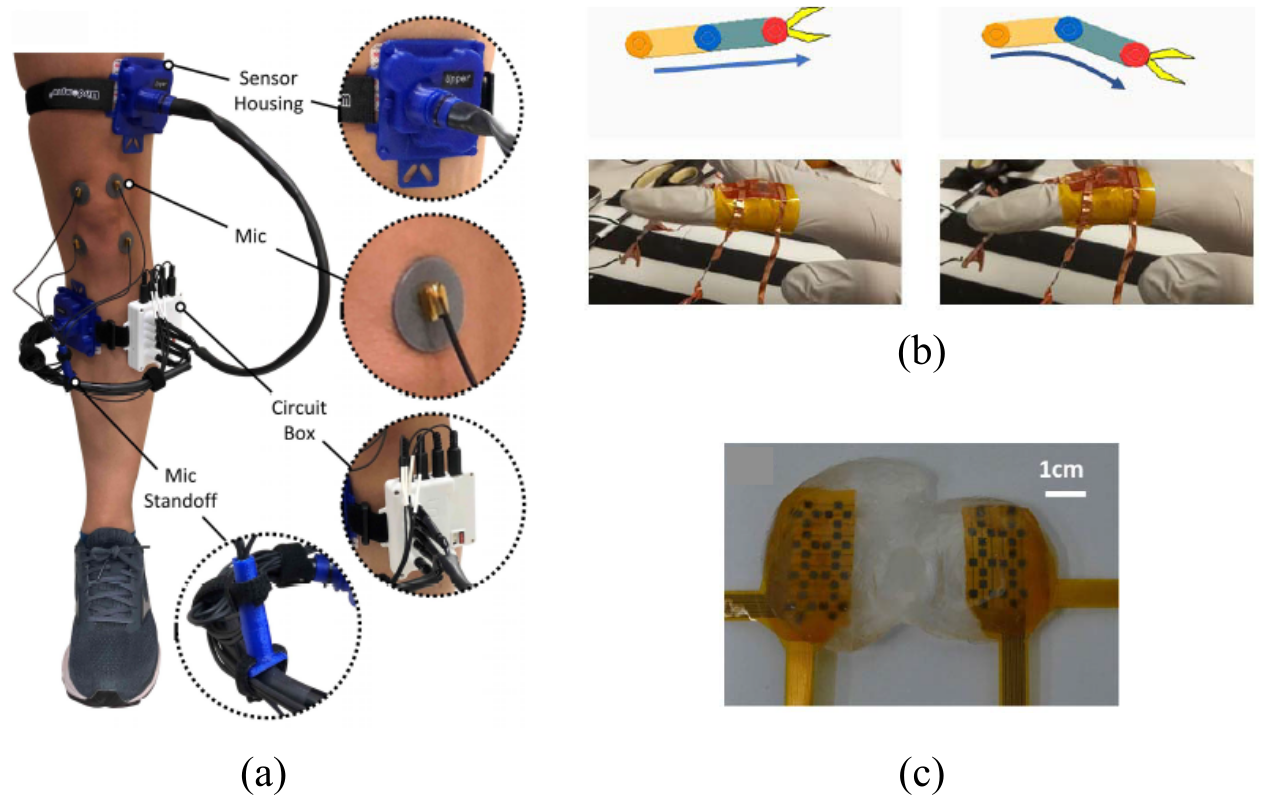
\includegraphics[scale=1]{Figure/Prosthetics/Prosthetics.png}
    \caption{Various assistive technologies used in prosthetics. (a) Wearable, multimodal sensor brace for knee joint health assessment, reproduced with permission from \parencite{teague_wearable_2020}.
     (b) A polymer microelectromechanical system-integrated flexible sensor, reproduced with permission from \parencite{fan_polymer_2019}.(c) A flexible pressure sensing device with bendable and distortable sensor arrays for force detection in knee arthroplasty, reproduced with permission from \parencite{sun_development_2020}.}
    \label{fig:Prosthetics}
\end{figure}

Another issue is the control of bionic hands. \textcite{alshammary_synergistic_2018} proposes using an inertial measurement unit (IMU) and electromyography (EMG) sensor for controlling a transhumeral myoelectric prosthesis, a type of bionic hand combined with a prosthetic forearm. The prosthetic system switches between hand- and elbow-based movement control dynamically according to the data from the IMU and the EMG sensors. The IMU on the forearm measures the angular velocity parallel to the elbow’s axis of rotation, and EMG electrodes on the upper to monitor muscular activity. When the elbow velocity is zero, and there is no upper arm activity, the control is given to the hand; when those parameters become non-zero again, the elbow takes control of the system. 



\subsection{Sensor in Use}
\subsubsection{Pressure Sensors}

Piezoresistive materials \parencite{sun_development_2020}, magnetic sensors \parencite{wu_skin-inspired_2018}, and MEMS-based sensors \parencite{fan_polymer_2019} are among the devices used for pressure sensing. The meniscus-shaped flexible pressure sensor in \textcite{sun_development_2020} is composed of polyimide (PI) electronic layers and nanocomposite sensing elements made of carbon nanotubes (CNT) and polydimethylsiloxane (PDMS). The size of the sensor is 2x2 $mm^2$ and it has a thickness of 400 $\mu$m. Due to the applied pressure, when deformation occurs on the sensing elements, the conductive channels  in CNTs increase. This reflects the external pressure change as a voltage variation at the sensor's output with 1\%/N sensitivity in the range of 10-100N.  

(Wu et al., 2018) makes use of PDMS as well for pressure detection. The sensor in \textcite{wu_skin-inspired_2018} is a PDMS chamber with magnetic particles deposited on top and an inductive sensing element located at the bottom of the chamber. An LC oscillation circuit is utilized as the sensing element. A 100-$\mu$m inductor wound around a coplanar waveguide of 60-$\mu$m thickness forms the inductor. With a force applied on the magnetic top layer (the sensing area is approximately $4x10^-5$ $m^2$), the distance between the the magnetic particles and the inductor changes, which in turn varies the LC oscillation frequency. The variations in the frequency can be translated into pressure changes of down to 10 $\mu$N. 

The MEMS device in \textcite{fan_polymer_2019} is another PDMS-based sensor that produces a variable current output proportional to the external pressure. The sensor is a $\mu$m-size capsule which top layer is encapsulated by a PDMS microstructure with three electrodes. When a pressure is applied on the capsule (whether on the top or bottom layers), the electrodes create contact with the patterned gold electrodes on the polyimide bottom layer. As the pressure increases, the quality of connection improves; therefore, the current flowing through the microstructure increases.

%%%%%%%%%%%%%%%%%%%%%%%%%%%%%%%%%%%%%%%%%%%%%%%%%%%%%%%%%%%%%%%%%%%%%%%%%%%%%%%%%%%%%%%%%%%%%%%%%%%%%%%%%%%%%%%%%%%%%%

\section{Brain-Computer Interface}
Due to the broad spectrum of cognitive disorders caused by neurological degradation due to old age or disease, cognitive-aids can be classified in many different categories. One major cognitive-aid category is Brain-Computer Interfaces (BCIs). In a broad sense, BCIs are used to infer volitional thought processes of their users and convert them into accessible signals. These signals can be used by an external device or other humans in the case of communications. To this end, devices record brain activity and generally apply some post-processing to generate a signal useful for another application. BCIs can either be noninvasive or invasive. Noninvasive devices typically use EEG sensors while invasive devices incorporate ECoG and ____ sensors. 

--Invasive BCIs and Non-Invasive BCIs reorganize the paragraphs.

\subsection{Brain-Computer Interface}
\begin{figure}[t]
    \centering
    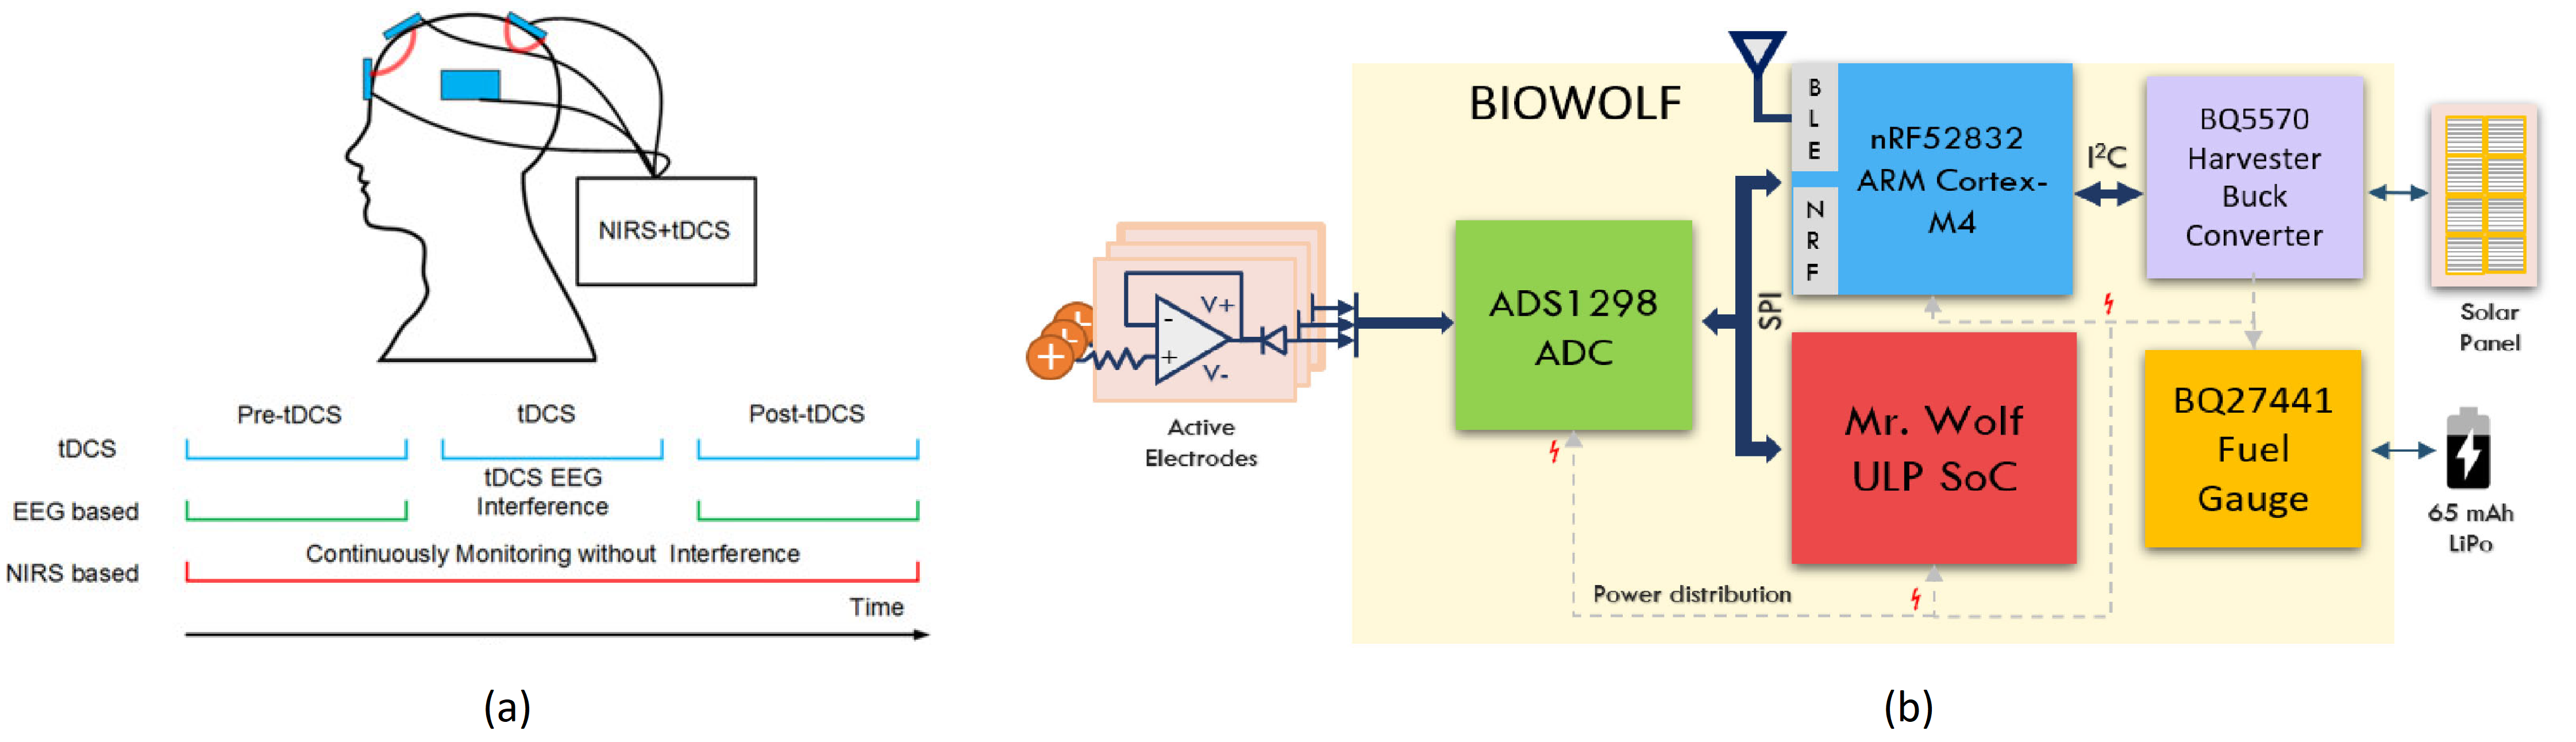
\includegraphics[width=\textwidth]{Figure/CognitiveAid/BCIcollage3}
    \caption{Brain-machine interface devices. (a) Illustration given in \textcite{miao_cmos-based_2018} of NIRS and tDCS systems integrated with different configurations that can be applied due to lack of cross-coupling. (b) Illustration given in \textcite{kartsch_biowolf_2019} of BioWolf system block diagram.}
    \label{fig:BCICollage}
\end{figure}
\textcite{lin_review_2010} characterizes 32 BCI devices based on seven design attributes of which four are described here. The first attribute, transmission media, looks at whether the system is wired or wireless. The next attribute, target users, infers the system application based on the study that the authors presented in their paper. If the study was conducted with healthy participants, it can be inferred that the system is for general commercial use. On the other hand, if the study participants have a specific disability then the that subgroup is concluded as the target users. The third attribute, sensor placement, refers to whether invasive ECoG electrodes or noninvasive EEG electrodes are used. Lastly, the neurological phenomenon attribute references the signal trend or phenomenon that is `detected' in post-processing to trigger the next stage. For example, one of the reviewed BCI systems by \textcite{ming_cheng_design_2002} uses steady-state visual evoked potentials (SSVEP) to identify user button selection on a virtual telephone keypad. In this case, the neurological phenomenon that triggers the keypad dialing is the SSVEP.

\textcite{miao_cmos-based_2018} presents a noninvasive BCI that uses transcranial direct-current stimulation (tDCS) with dynamic dosage adjustment. tDCS is a noninvasive approach that uses electrodes connected to the skull for stimulation. In prior work \parencite{roh_wearable_2014}, devices using tDCS ran into dynamic stimulation adjustment issues because of electroencephalogram (EEG)-based closed-loop techniques coupled with the electrical stimulation mechanism. The proposed device in \textcite{miao_cmos-based_2018} uses frequency-domain near-infrared spectroscopy (fdNIRS) that side-steps the issue of electrical coupling by using optical recording as part of the feedback mechanism. Sensing of cerebral hemodynamics is done with signal processing techniques applied on a fdNIRS signal captured by a simple avalanche photodiode. 

\textcite{kartsch_biowolf_2019} proposes a BCI device that tackles a primary limiting factor in the wide adoption of BCIs, which is inadequate battery life and processing power. An improvement in one of these areas results in a reduction in the other. \textcite{kartsch_biowolf_2019} proposes a novel parallel digital signal processing (DSP) chip and microcontroller architecture that increases the processing power while simultaneously keeping system power consumption low. The system directly converts brain signals collected by active electrodes into digital signals via a commercial analog-to-digital converter. The resulting signal is fed into a parallel ultra-low-power system-on-a-chip (SoC) designed by the authors in \textcite{pullini_mr_2018} dubbed Mr.Wolf. The Mr.Wolf SoC uses nine RISC-V processors arranged in parallel optimized with additional hardware to implement DSP algorithms. The resulting non-invasive system along with a solar energy harvester and a commercial low-power RF communication chip were tested on five healthy subjects. The results showed that the device battery life was up to 38 hours.

\textcite{zhou_hybrid_2020} explores ways to improve the performance of BCIs by combining  EOG- and SSVEP-based eye trackers. SSVEP-based eye trackers are asynchronous BCIs that have a major drawback of not being able to distinguish between an idle and a control state. Eyeblink detection in EOG sensory can overcome the mentioned challenge of SSVEP. In the combined system, while SSVEP signals determine whether the user's eye focuses on the control button, the EOG sensory detects the user's eye blinks. The only case that issues a command in the control state is when the user pays attention to the command button and blinks an eye. This method effectively reduces the false-positive rate (FPR). While wearable EEG electrodes on the user's head record the SSVEP signals, a single electrode on the forehead monitors the EOG signal along with a reference electrode on the right mastoid. To test the command accuracy and FPR,  ten subjects with healthy vision participated in free spelling experiments. The free spelling test requires each subject to select 48 predefined characters and then remain in the idle state for 10 minutes. The achieved performance of the proposed hybrid BCI is 95.42\% $\pm$ 2.15\% accuracy and 0.80\% $\pm$ 0.75\% FPR. Testing with the same subjects using conventional SSVEP based BCIs resulted in a slightly worse accuracy of 94.58\% $\pm$ 7.16\% and a higher FPR of 12.77\% $\pm$ 8.55\% which shows the positive impact of the eye trackers used in the proposed BCI. 

\textcite{deng_bayesian_2020} explores the applications of SSVEP further by taking advantage of another SSVEP eye tracking application. SSVEP develops in the visual cortex when a subject focuses on a flickering visual stimulus \parencite{nakanishi_high-speed_2014}. SSVEP signals are extracted from EEG signals and utilized to issue a control command of the environment. \textcite{deng_bayesian_2020} presents a Bayesian-shared-control human-machine interface to control a smart wheelchair using this form of eye tracking. The system integrates a stimuli module consisting of 4 LEDs where each LED represents one command. The wheelchair direction control options are move forward, slow down, turn left, and turn right. The wheelchair turn angle choices range from 0$^{\circ}$ to  90$^{\circ}$ in 30$^{\circ}$ increments. As the stimulus paradigm is two-layer, the user needs to command a direction before an angle command. When the user's eye focuses on either LED, the SSVEP signals will respond, and the related control command will be issued. The experiments were performed with eleven healthy subjects to test the wheelchair motion controls'  accuracy through the proposed BSC-HMI. For the online test, each subject was required to control the wheelchair passing along a particular route five times. The average statistical reliability of BSC-HMI was 71.82\%.  A deep learning approach is planned to be employed to decode EEG signals and apply various stimulus paradigms as the next step of this work to reduce the latency.

%%%%%%%%%%%%%%%%%%%%%%%%%%%%%%%%%%%%%%%%%%%%%%%%%%%%%%%%%%%%%%%%% SECTION REMOVED %%%%%%%%%%%%%%%%%%%%%%%%%%%%%%%%%%%%%%

% \subsection{General Cognitive Aids}
% \begin{figure}[t]
%     \centering
%     \includegraphics[width=\textwidth]{Figure/CognitiveAid/GCACollage3}
%     \caption{General cognitive aids. (a) Illustration given in \textcite{jia_mm-sized_2020} of optical and electrical stimulation headstage and implanted device in a rat. (b) Microscopic photograph given in \textcite{yamakawa_implantable_2019} of the fabricated probe head with ECoG, temperature, and photodiode sensors}
%     \label{fig:GCACollage}
% \end{figure}
% BCI devices are not the only form of cognitive aids. There are a plethora of devices that perform functions such as invasive and non-invasive measurement of signals correlated with brain activity as well as both optical and electrical stimulation of the brain. 
% %But, they are not meant to act as BCIs. 
% For instance, \textcite{yamakawa_implantable_2019} presents an implantable flexible strip device designed to measure brain temperature, electrical activity, and oxygenation levels during surgery. Brain temperature is measured using a simple negative temperature coefficient thermistor. Six-channel platinum ECoG electrodes record the electrical activity. The oxygenation levels are determined by shining a light on the tissue and analyzing the change in amplitude and phase of the reflected signal. Since the flexible string is only used during surgery, the system lacks a wireless data transfer module. However, this device shows the promise of integrating three relevant sensing modalities; therefore, it could lead to future research in the design of wireless, permanently implanted devices similar to this one. 

% \textcite{jia_mm-sized_2020} proposes a monitoring system, where the sensing portion is implanted and the data is wirelessly transmitted to an external source. The system can stimulate the brain by both electrical and optical stimulation mechanisms and also close the loop with neural recording. Despite being less power efficient, the advantage of optical stimulation is that it is cell type-specific. As a way to benefit from the best of both stimulation modalities, \textcite{jia_mm-sized_2020} presents a device that offers 16-channel optical and 4-channel electrical stimulation. The proposed device consists of a headstage and one or more small implantable modules, called free-floating wireless implantable optoelectric stimulators (FF-WIOS2). The headstage communicates via low-energy Bluetooth to external devices as well as by inductive link to one or more FF-WIOS2 using on-off keying. Each FF-WIOS2 device has electrodes for electrical stimulation and uLEDs for optical stimulation. 

% Moving away from monitoring different brain signals, there is also a whole field dedicated to stimulation. Stimulation of the brain is a proven treatment for some neurological disorders that affect movements. \textcite{amon_systems_2017} reviews and compares many commercially available Deep Brain Stimulators (DBSs) produced mainly by Boston Scientific (B), Medtronic (M), and St. Jude (S). Reviews are based on a variety of technical considerations including electrical source, number of implantable pulse generators (IPGs), electrode design, polarity, and electrical stimulation signal. According to the review, B devices offered current source stimulation to avoid issues with impedance changes that affect stimulation current. B devices also have more than one IPG to enable stimulation of each hemisphere of the brain separately if desired. Segmented eight electrode design with multi-polar configurations was also used by B devices. Finally, many stimulation configurations offered by B devices allow the treatment of different symptoms and limit unwanted side effects of stimulation outside the localized region. S devices also provide the same features as the B devices except for not being able to set different amplitude levels for each contact during stimulation. M devices varied mainly in electrode design, where their systems were equipped with classic unipolar ring contact electrodes. They also shared the S device characteristic of being designed with a single current source in contrast to B devices.

%%%%%%%%%%%%%%%%%%%%%%%%%%%%%%%%%%%%%%%%%%%%%%%%%%%%%%%%%%%%%%%%%%%%%%%%%%%%%%%%%%%%%%%%%%%%%%%%%%%%%%%%%%%%%%%%%%%%%%%%

\subsection{Sensors In Use}
This section will highlight sensors that are distinct to the cognitive aid field. However, it should be noted that there are many redundant sensors in use with cognitive aids that are not highlighted since they have been discussed in previous sections.

% \subsubsection{Platinum ECoG Electrodes}
% Platinum electrodes are among metals that do not participate in the sensing chemical reaction. As a result, they are more stable and well suited for amperometric (i.e., current) sensing \parencite{ida_sensors_2013}. These types of sensors are referred to as ``polarizable'' electrodes. In \textcite{yamakawa_implantable_2019}, platinum electrodes are used to measure ECoG signals during brain surgery.

% \subsubsection{NTC Thermistors}
% Thermistors are generally made of a semiconducting material that has a high temperature coefficient. The material resistance changes with respect to temperature in a non-linear manner \parencite{ida_sensors_2013}. The proportionality of resistance to temperature can either be direct or inverse, depending on the sign of the temperature coefficient, i.e. positive temperature coefficient (PTC) or negative temperature coefficient (NTC). In \textcite{yamakawa_implantable_2019}, an NTC thermistor is used to measure the surface temperature of the cerebral cortex during brain surgery. 

% \subsubsection{Avalanche Photodiodes}
% Avalanche photodiodes are a subcategory of photodiodes that take advantage of the avalanche effect to act as photomultiplier sensors \textcite{ida_sensors_2013}. As a result, these photodiodes are more sensitive than photoconductive mode diodes, more advantageous in certain applications. For example, in \textcite{miao_cmos-based_2018} the system requires the detection of photocurrents as small as 10 nA. For this example, avalanche photodiodes are used due to their high sensitivity.  


%%%%% These are from Yifei's section. Aatreya, these are more relavant to your section. Could you please blend in?

%\subsubsection{Electrode}

%Electrodes are used for EEG and EOG signals detection. As GKP and SSVEP levels are potential alteration of the EEG signals, EEG active %electrodes can effectively detect GKP and SSVEP levels. 
%A commercial biopotential measurement system with active electrodes, Biosemi ActiveTwo, is used in (Nam et al., 2016) for SSVEP potential level %detection. Biosemi ActiveTwo is capable of recording from up to 264 electrodes with a maximum 16 kHz sampling rate. This study uses 33 %electrodes with a sampling rate of 2048 Hz. The user wearing a set of electrodes on Biosemi ActiveTwo could control a powered wheelchair %through the proposed TDS.
\section{Conclusion}
\lipsum[1]
%%%%%%%%%%%%%%%%%%%%%%%%%%%%%%%%%%%%%%%%%%%%%%%%





%\bibliographystyle{harvard}
% argument is your BibTeX string definitions and bibliography database(s)


\printbibliography

% can use a bibliography generated by BibTeX as a .bbl file
% BibTeX documentation can be easily obtained at:
% http://mirror.ctan.org/biblio/bibtex/contrib/doc/


% biography section
% 
% If you have an EPS/PDF photo (graphicx package needed) extra braces are
% needed around the contents of the optional argument to biography to prevent
% the LaTeX parser from getting confused when it sees the complicated
% \includegraphics command within an optional argument. (You could create
% your own custom macro containing the \includegraphics command to make things
% simpler here.)
%\begin{IEEEbiography}[{\includegraphics[width=1in,height=1.25in,clip,keepaspectratio]{mshell}}]{Michael Shell}
% or if you just want to reserve a space for a photo:

% \begin{IEEEbiography}{Ulkuhan Guler}
% Biography text here.
% \end{IEEEbiography}

% \begin{IEEEbiography}{Maysam Ghovanloo}
% Biography text here.
% \end{IEEEbiography}

% if you will not have a photo at all:
% \begin{IEEEbiographynophoto}{Maysam Ghovanloo}
% Biography text here.
% \end{IEEEbiographynophoto}


% You can push biographies down or up by placing
% a \vfill before or after them. The appropriate
% use of \vfill depends on what kind of text is
% on the last page and whether or not the columns
% are being equalized.

%\vfill

% Can be used to pull up biographies so that the bottom of the last one
% is flush with the other column.
%\enlargethispage{-5in}

% that's all folks
\end{document}
